\documentclass[a4paper,fleqn]{cas-sc}
\usepackage[utf8]{inputenc}
\usepackage{CJKutf8}
\usepackage[authoryear,longnamesfirst]{natbib}
\usepackage{booktabs}
\usepackage{amsmath}
\usepackage{amssymb}
\usepackage{bm}
\usepackage{graphicx}
\usepackage{hyperref}

\begin{document}
\begin{CJK*}{UTF8}{gbsn}
\let\WriteBookmarks\relax
\def\floatpagepagefraction{1}
\def\textpagefraction{.001}

\title{面向长时程多智能体大语言模型系统的上下文治理与长期记忆图谱方法研究}
\date{}

\maketitle

\begin{abstract}
随着大语言模型智能体逐步从单轮问答工具演化为能够规划、检索、工具调用、跨轮协作并持续保持状态的长时程系统，研究焦点已经不再只是“模型能否回答”，而是“系统如何在有限提示预算下稳定运行”。本研究据此将问题正式拆解为两个可独立建模、又可系统集成的研究单元：其一是受象群族长记忆启发的多智能体上下文治理方法，用于决定当前运行中哪些上下文应被保留、压缩或舍弃；其二是受克拉克星鸦空间记忆与藏食回收行为启发的长时记忆图谱机制，用于决定哪些执行经验应被提升为长期记忆、如何组织为记忆胶囊节点与关系边，以及未来如何按线索召回相关子图。

围绕这一目标，本文将统一框架重写为“大象-星鸦框架”（Elephant-Nutcracker Framework）。其中，大象注意力负责运行内显著性治理与预算约束下的上下文管理；克拉克星鸦长时记忆图谱机制负责跨运行长期记忆的表示、组织与检索返回；MGCM 继续承担治理层角色，负责记忆候选的提升、验证、降级与废弃，而不直接承担图谱表示；长时程注意力、上下文压缩与事件中心可观测性则共同支持系统连续执行、提示构造与机制解释。与原有“图谱化长期记忆”叙述不同，本文强调长期记忆应作为即插即用模块存在：它可以独立接入现有 AgentOrch 运行时，通过标准接口接收候选记忆胶囊，并返回可注入提示的局部子图或子图摘要。

在论文组织上，本文不再将统一稿件视为单篇方法文章，而是将其重构为一个大论文总论与两篇章节论文：第三章聚焦象群启发的上下文管理，第四章聚焦克拉克星鸦长时记忆图谱机制，第五章再对两者进行系统融合与综合实验验证。当前仓库中的 \texttt{seagull\_memory}、\texttt{rq3\_seagull\_memory} 等命名仅作为历史实现别名保留，用于对齐既有实验资产；主文中的理论命名统一采用“克拉克星鸦长时记忆图谱机制”。
\end{abstract}

\noindent\textbf{关键词：} 大语言模型智能体；多智能体系统；大象注意力；克拉克星鸦长时记忆图谱；上下文治理；长时程推理；MGCM；事件中心可观测性。

\section{引言}

大语言模型正迅速从单轮文本生成器演化为能够规划、检索、调用工具、与外部软件协同并在长时间跨度内维持任务状态的自主系统。关于自主智能体与大语言模型多智能体系统的正式综述表明，这类系统的实际能力已不再仅仅取决于底层模型本身，还取决于其外围的智能体栈如何组织角色分工、通信、记忆、工具使用与环境交互 \citep{wang2024survey,guo2024llmmas,li2024masworkflow}。在 2019--2026 年的研究脉络中，这一演化在 2023 年之后尤其明显：系统逐步从单智能体闭环执行扩展为由多个具备角色、记忆与工具接口的智能体组成的协作系统，并在软件开发、社会模拟与交互环境评测等方向形成了较成熟的工程范式 \citep{hong2024metagpt,qian2024chatdev,liu2024agentbench,zhou2024sotopia}。当任务超出一次提示-响应循环时，这种转变尤为明显。长篇研究、编码、分析或多阶段执行都要求系统在大量决策、工具调用、子任务交接与延迟反馈中保持稳定。在这种场景下，单智能体提示和朴素的长上下文累积会变得愈发脆弱。

其核心困难并不仅仅来自规模，而是来自耦合治理。长时程多智能体系统至少面临四类相互依赖的挑战。第一，协作会带来协调压力：系统必须决定由哪个智能体执行、应交接哪些上下文，以及专业化输出如何影响集体行为。第二，长期运行会带来记忆压力：系统必须决定哪些内容应保持短暂、哪些应提升为共享记忆，以及哪些值得跨运行持久保存。第三，有限提示预算会带来压缩压力：候选上下文几乎总是超过可用提示容量。第四，扩展执行会带来可观测性压力：如果没有结构化轨迹，便很难诊断失败、估计成本，甚至难以重建一次运行中究竟发生了什么。

现有研究确实覆盖了该问题的重要部分，但很少将其统一起来。第一条主线是单智能体闭环执行与反馈学习，重点强调规划、工具使用和反思纠错 \citep{wang2024survey,yao2023react,shinn2023reflexion}。第二条主线是 LLM 多智能体架构与协作机制，围绕角色专门化、任务分解、结构化通信与系统扩展展开，并已经形成从早期角色扮演到大规模协作网络的连续谱 \citep{guo2024llmmas,li2024masworkflow,li2023camel,wu2023autogen,hong2024metagpt,qian2024chatdev,gan2025master,wang2025megaagent,qian2025macnet,du2025crossteam}。第三条主线是系统级评测、社会交互与长期记忆治理，研究者开始从交互环境、社会智能与鲁棒性角度评估多智能体系统，而不再只看静态任务分数 \citep{liu2024agentbench,chan2024chateval,zhou2024sotopia,wang2024sotopiapi,dong2026pear}。与此同时，长上下文建模、检索增强与记忆架构为长时程执行提供了关键使能条件 \citep{li2024sbarope,lewis2020rag,park2023generative}。然而，这些方向往往仍以模块化附加件形式存在。现有文献仍缺少一种统一方法，将协作显著性、长期记忆图谱、长时程连续性以及预算约束下的上下文压缩视为同一治理框架的组成部分。

本文正是为此提出统一框架。我们引入大象注意力作为系统级策略，用于在运行过程中优先保留经过验证且具有社会性意义的上下文；引入克拉克星鸦长时记忆图谱机制作为互补机制，用于让高价值经验跨运行提升为长期记忆胶囊，并在未来条件满足时按子图形式返回复用。随后，我们将这两者置于更大的方法框架中，并加入长时程注意力以维持长轨迹上的执行连续性，以及上下文压缩以处理预算约束下的提示构造。为使闭环更加明确，我们还将这些机制与 MGCM 及事件中心可观测层整合，用于把执行轨迹投影为可解释的 todo 状态，并为记忆治理提供结构化证据。

本文的主要贡献体现在四个彼此衔接的方面。首先，我们提出 \textbf{大象注意力}，把多智能体执行中的上下文保留从单纯的新近性偏好重新分配到已验证、可复用且具有社会性意义的信息上。其次，我们提出 \textbf{克拉克星鸦长时记忆图谱机制}，将跨运行、跨线程的记忆提升、图谱化表示与子图返回过程形式化，而不再把长期记忆视为简单的对话累积。再次，我们给出一个 \textbf{统一的长时程方法框架}，在预算感知的统一表述下把大象注意力、克拉克星鸦长时记忆图谱机制、长时程注意力与上下文压缩纳入同一体系。最后，我们定义一个 \textbf{事件中心可观测性与评估框架}，把 MGCM、运行事件与 todo 投影连接起来，使调试、可解释分析与后续经验验证可以建立在同一套结构化证据之上。
从论文组织上看，当前统一框架将被进一步拆解为两个可独立成文、又能在系统层整合的研究单元：一是象群族长记忆启发的多智能体上下文管理方法，二是克拉克星鸦长时记忆图谱机制。这一拆解既服务于硕士论文的章节化结构，也使每个模块能够拥有独立研究问题、实验协议与结论边界。

\section{相关工作}

\subsection{大语言模型自主智能体}

大语言模型自主智能体通常被建模为在推理、行动与环境反馈之间交替循环的系统，而非一次性文本生成器。综述工作强调了规划、记忆、动作模块与自我反思等组件的重要性 \citep{wang2024survey}。ReAct 展示了将推理轨迹与面向工具的行动显式耦合的价值 \citep{yao2023react}，而 Reflexion 则引入了基于执行反馈的语言式自我改进 \citep{shinn2023reflexion}。这些工作奠定了基础，因为它们说明了系统性能依赖于结构化执行闭环。然而，它们主要聚焦于单智能体行为，并未完整说明在长时程多智能体场景下，跨角色上下文选择、跨运行长期记忆图谱与预算感知可观测性应如何被统一治理。

\subsection{基于大语言模型的多智能体系统}

作为经典基础背景，Wooldridge 对多智能体系统中的协作、协调与组织结构给出了非 LLM 时代的系统框架 \citep{wooldridge2009}。在 LLM 语境下，正式综述已经把研究重点推进到基于角色画像、通信模式、环境接口和能力获取机制的系统设计 \citep{guo2024llmmas,li2024masworkflow}。代表性系统方面，CAMEL 通过角色扮演机制展示了多智能体协作与数据生成的可行性 \citep{li2023camel}；AutoGen 将可对话智能体与群聊编排抽象为通用框架，是少数仍值得保留的高影响预印本代表 \citep{wu2023autogen}；MetaGPT 和 ChatDev 分别将 SOP、结构化消息与软件开发流水线纳入协作骨架，推动了软件工程场景中的多智能体系统化设计 \citep{hong2024metagpt,qian2024chatdev}。进一步地，MASTER 以 LLM specialized MCTS 组织招募与通信，MegaAgent 探索了无预定义 SOP 的大规模自治协作，Scaling Large Language Model-based Multi-Agent Collaboration 研究了多智能体协作的规模扩展规律，而 Cross-Team Orchestration 则把多团队并行探索与阶段性交叉协作正式化 \citep{gan2025master,wang2025megaagent,qian2025macnet,du2025crossteam}。这些工作极大丰富了协作范式，但研究重点仍多落在流程设计、角色编排或团队扩展上，对跨智能体上下文传播、记忆提升与事件化证据治理的讨论仍然不足。

\subsection{评测、社会交互与系统比较}

系统级评测正在从静态任务分数转向交互行为、社会智能与鲁棒性。AgentBench 将评测对象从单步回答扩展到多环境交互，强调长程决策与行动能力 \citep{liu2024agentbench}。ChatEval 则通过多智能体辩论式评审模拟多人裁决过程，推动了 LLM-as-a-judge 从单评委到多评委机制的演进 \citep{chan2024chateval}。在社会交互场景中，SOTOPIA 构造了开放式社会情境来评估语言智能体的社会目标完成能力 \citep{zhou2024sotopia}，而 SOTOPIA-$\pi$ 进一步把交互式学习引入社会智能训练，并揭示了基于 LLM 的评审信号可能高估针对性训练模型的问题 \citep{wang2024sotopiapi}。最新的 PEAR 则把 planner--executor 架构的效用与脆弱性放到统一基准中考察，突出说明了多智能体系统不仅要比较最终任务结果，还要评估记忆配置、攻击面与鲁棒性权衡 \citep{dong2026pear}。这些工作说明，系统比较已经从“谁的分数更高”转向“谁在更真实的交互条件下更可靠、更安全、更可解释”。

\subsection{长上下文与长时程推理}

扩展上下文长度已成为重要研究方向，因为许多真实任务超出了朴素提示累积所能稳定处理的范围。围绕旋转位置编码变体等长上下文技术的研究，提升了模型在更大窗口下的表示鲁棒性 \citep{li2024sbarope}。然而，长时程执行并不能仅仅化约为上下文长度。即使一个系统拥有较长的上下文窗口，它仍可能失败，因为它无法保持过程连续性、无法区分高价值与低价值历史，或无法随时间维持一致的压缩状态。因此，我们将长时程推理视为一个运行时治理问题，而不仅仅是模型容量问题。也正是在这一点上，单纯“扩窗口”的技术路线与面向多智能体协作的上下文治理路线发生了分化。

\subsection{检索、记忆与上下文管理}

检索增强生成表明，访问外部知识能够显著改善知识密集型任务 \citep{lewis2020rag}。更广泛地说，智能体系统越来越依赖检索、情景记忆、工作空间产物与摘要机制来应对规模问题。Generative Agents 将记忆、反思与计划显式结合，展示了记忆架构对群体行为与长期连续性的决定性作用 \citep{park2023generative}。SOTOPIA-$\pi$ 说明交互式学习能够提升社会情境中的策略表现，但也暴露出评测信号与训练目标耦合的偏差 \citep{wang2024sotopiapi}。PEAR 则进一步表明，在 planner--executor 架构中，记忆放在规划者一侧比放在执行者一侧更关键，而且性能提升往往伴随鲁棒性权衡 \citep{dong2026pear}。然而，朴素累积通常会增加噪声，而简单检索也无法回答更难的问题：哪些内容应被持久化、哪些应被提升、以及哪些内容应在未来返回。我们的框架通过在同一方法流水线中联合建模运行中的显著性、治理化提升、图谱化长期存储以及预算约束压缩，与现有方法形成区别。

\subsection{本文工作的定位}

与已有研究相比，本文方法有三点关键区分。第一，它将运行内显著性治理与跨运行长期记忆图谱分离，并分别形式化为大象注意力与克拉克星鸦长时记忆图谱机制。第二，它将长时程连续性与上下文压缩视为在提示预算下耦合的优化问题，而不是若干启发式工具。第三，它将事件中心可观测性从工程层面的辅助监控提升为方法论基础设施，因为结构化轨迹能够支持进度投影、记忆治理与失败分析。换言之，本文并不是再发明一个通用的多智能体编排框架，而是提出一个治理导向的统一框架，补足现有系统在消息筛选、长期记忆图谱、长时程连续性和事件化证据上的共性空缺。

\section{问题表述}

我们考虑一个长时程多智能体大语言模型系统。它接收用户请求 $x$，运行于线程状态 $\mathcal{H}_t$ 中，拥有工具集合 $\mathcal{T}$、可检索知识底座 $\mathcal{R}$、可用智能体集合 $\mathcal{A}$，以及多个记忆存储层。在决策步 $t$，系统必须构造一个可执行提示上下文 $\mathcal{C}_t$，并从如下动作空间中选择动作 $a_t$：
\begin{equation}
\mathcal{U} = \mathcal{U}_{\text{reason}} \cup \mathcal{U}_{\text{tool}} \cup \mathcal{U}_{\text{retrieve}} \cup \mathcal{U}_{\text{delegate}} \cup \mathcal{U}_{\text{memory}}.
\end{equation}
这里，动作既可以是直接推理步骤，也可以是工具调用、检索请求、任务委派或记忆治理更新。

压缩之前的候选上下文为
\begin{equation}
\mathcal{X}_t = \mathcal{H}_t \cup \mathcal{M}^{\text{local}}_t \cup \mathcal{M}^{\text{collective}}_t \cup \mathcal{M}^{\text{nutcracker}}_t \cup \mathcal{R}_t \cup \mathcal{D}_t \cup \mathcal{S}_t,
\end{equation}
其中，$\mathcal{M}^{\text{local}}_t$ 表示局部工作记忆，$\mathcal{M}^{\text{collective}}_t$ 表示受治理的共享记忆，$\mathcal{M}^{\text{nutcracker}}_t$ 表示来自历史运行并在当前返回的星鸦长期记忆图谱胶囊候选，$\mathcal{R}_t$ 表示检索到的证据，$\mathcal{D}_t$ 表示委派数据包与协调元数据，$\mathcal{S}_t$ 表示策略指令或结构化控制片段。

提示构造受有限 token 或字符预算 $B_t$ 约束。令每个候选片段 $z_i \in \mathcal{X}_t$ 的大小为 $\ell_i$，则提示构造器必须选择子集 $\mathcal{C}_t \subseteq \mathcal{X}_t$，满足
\begin{equation}
\sum_{z_i \in \mathcal{C}_t} \ell_i \leq B_t.
\end{equation}
因此，上下文构造被转化为受约束的选择问题，而非追加式对话堆积问题。

多智能体执行还引入了路由策略
\begin{equation}
\pi_{\text{route}} : (x, \mathcal{H}_t, \mathcal{X}_t) \mapsto \{(\alpha_j, \tau_j)\}_{j=1}^{m_t},
\end{equation}
其中 $\alpha_j \in \mathcal{A}$ 是被选中的智能体，$\tau_j$ 是紧凑任务数据包。系统不仅要决定由谁执行，还要决定应随委派携带哪些压缩后的上下文与记忆证据。

记忆在四个层级上受到治理：
\begin{equation}
\mathcal{M}_t = \{\mathcal{M}^{\text{local}}_t, \mathcal{M}^{\text{candidate}}_t, \mathcal{M}^{\text{collective}}_t, \mathcal{M}^{\text{nutcracker}}_t\}.
\end{equation}
其中，局部记忆服务于当前运行；候选记忆存放尚未验证的中间知识；集体记忆存放已验证的共享知识；星鸦图谱记忆存放可在未来以子图形式返回的跨运行长期记忆胶囊。

最后，执行过程会产生事件流
\begin{equation}
\mathcal{E} = (e_1, e_2, \ldots, e_T),
\end{equation}
其中每个事件都包含诸如 run ID、thread ID、task ID、阶段与元数据等标识。这些事件并不是附属产物，而是形式化研究对象的一部分，因为它们同时支持运行时可观测性与基于事件的 todo 投影。

在这一表述下，研究问题可以归结为：设计一族统一策略
\begin{equation}
\Pi = \{\pi_{\text{elephant}}, \pi_{\text{nutcracker}}, \pi_{\text{horizon}}, \pi_{\text{compress}}, \pi_{\text{mgcm}}, \pi_{\text{obs}}\}
\end{equation}
以便在有限上下文预算与多步执行条件下，提高长时程多智能体系统的性能、连续性与可解释性。

\section{方法}

\subsection{总体框架}

本文提出的大象-星鸦框架是一种面向长时程多智能体大语言模型系统的统一运行时方法。其执行流程可概括为
\begin{equation}
x \rightarrow \text{路由} \rightarrow \text{上下文构造} \rightarrow \text{推理/委派} \rightarrow \text{工具/检索执行} \rightarrow \text{记忆提升/图谱写入} \rightarrow \text{可观测性投影}.
\end{equation}

给定请求 $x$ 后，系统首先解析路由策略，决定任务是保持单智能体执行、进入工作流，还是委派给专业化智能体。随后，系统从线程历史、记忆层、检索证据、策略指令与委派数据包中构造候选上下文。大象注意力与上下文压缩共同决定在当前提示预算下哪些片段能够保留下来。活跃智能体或监督者随后基于压缩后的提示进行推理，在需要时调用工具或检索，也可继续拆分并委派子任务。执行结束后，MGCM 决定产生的知识是保留在本地、成为候选共享笔记，还是被提升为集体记忆。随后，克拉克星鸦长时记忆图谱机制进一步决定哪些高价值经验应被提升为跨运行长期记忆胶囊，并在何种线索与约束下以子图形式返回。与此同时，所有执行阶段都会产生结构化事件，并被持久化与投影到 todo 视图中，用于进度重建。

这种表述使该框架成为一种以方法为中心、而非以架构为中心的方案。重点不在于枚举软件模块，而在于明确规定上下文、记忆与协作如何跨时间被联合治理。

从论文结构映射的角度看，尽管当前主稿仍采用期刊式的 \verb|\section|/\verb|\subsection| 组织方式，但其方法论实际上被拆解为两个边界清晰的研究单元。前一单元对应第三章的群体上下文治理问题，关注多智能体系统在单次运行中如何从线程历史、工具观测、委派数据包与共享记忆中筛选、压缩并路由最有价值的上下文；后一单元对应第四章的个体长期记忆问题，关注单个经验如何经由治理被提升为可跨运行复用的长期记忆胶囊，并进一步组织为可检索子图。换言之，个体记忆是底层知识来源，群体记忆是这些来源在当前运行中经过治理后的共享结果。本文在本节先给出统一框架，再分别展开第三章与第四章所对应的两类机制。

\subsection{大象注意力}

从章节化研究问题看，大象注意力对应本文第三章的核心机制。该章并不试图同时解决“当前应看什么”和“未来应记住什么”这两类问题，而是聚焦于预算受限条件下的群体上下文治理：当多个智能体、工具输出和中间产物同时竞争有限提示空间时，系统应如何决定哪些信息进入当前提示、哪些只保留为候选共享记忆、哪些被压缩延后，乃至哪些应被直接舍弃。因此，本节关注的是共享上下文的显著性排序、跨角色传播与协作稳定性；个体长期记忆的形成、表示与跨运行返回不作为本节重点，而作为下一部分以及论文第四章的独立研究对象展开。

大象注意力并不是神经网络内部的注意力层，而是一种系统级显著性策略，用于在协作执行中对候选上下文进行耐久性重要度排序。对于每个候选片段 $z_i \in \mathcal{X}_t$，定义其大象注意力分数为
\begin{equation}
s_i^{\text{EA}} = \alpha \, \mathrm{Rel}(z_i, x) + \beta \, \mathrm{Val}(z_i) + \gamma \, \mathrm{Reuse}(z_i) + \delta \, \mathrm{Out}(z_i) - \lambda \, \mathrm{Red}(z_i),
\end{equation}
其中 $\mathrm{Rel}$ 衡量任务相关性，$\mathrm{Val}$ 衡量验证支持程度，$\mathrm{Reuse}$ 衡量跨运行或跨智能体的复用程度，$\mathrm{Out}$ 衡量其与成功结果的关联，$\mathrm{Red}$ 则用于惩罚冗余。

大象注意力的治理偏置可写为
\begin{equation}
\beta + \gamma + \delta > \alpha_{\text{recency}},
\end{equation}
这表示经过验证、可复用并受到结果支持的上下文，能够压过仅仅“最新”的上下文。这一点不同于以新近性为主导的提示组装方式，后者往往会高估新近但不稳定的交互历史。

在实践中，大象注意力要解决的是一个典型的协作问题：当多个智能体、工具输出与中间结果争夺有限提示预算时，什么应当持续保持影响力。当专业化智能体的产出与已验证规则需要在后续决策中持续发挥作用时，该机制尤为重要。

\subsection{克拉克星鸦长时记忆图谱机制}

仅有运行内的群体上下文治理仍不足以支撑长时程系统的跨线程适应。大象注意力能够回答“当前这一轮什么最该被看见”，却不能单独回答“哪些经验值得被长期保存、未来如何按线索召回，以及如何避免陈旧或冲突记忆重新污染当前提示”。因此，在群体治理层之上，还需要一个面向个体经验沉淀与长期复用的记忆机制。前一部分解决的是运行内共享上下文的选择问题，后一部分解决的是跨运行个体经验的存储与返回问题，二者共同构成长时程多智能体系统的记忆闭环。

从论文组织上看，克拉克星鸦长时记忆图谱机制对应第四章。该章的研究对象不再是多个智能体在当前运行中的上下文竞争，而是单个经验单元如何从局部工作痕迹演化为可复用的长期记忆胶囊。围绕这一目标，本文重点考察四个相互衔接的环节：经验抽取与规范化表示、基于验证与复用信号的提升判定、图谱节点与关系边构建，以及面向后续任务的安全返回与子图注入。也就是说，本节关注的是个体长期记忆的形成、表示、检索与更新；这些个体记忆在返回到运行时之后，才进一步参与上一节所讨论的群体上下文治理。

克拉克星鸦长时记忆图谱机制负责长期记忆胶囊的图谱化表示、组织与返回检索。它与大象注意力的目标不同。大象注意力关注的是当前运行期间哪些上下文更重要；而克拉克星鸦长时记忆图谱机制关注的是哪些经验值得被提升为长期记忆、如何被表示为记忆胶囊节点并通过关系边连接，以及未来在何种线索下应按子图形式安全返回。

对于一个记忆候选 $m$，定义其提升分数为
\begin{equation}
\mu(m) = \rho_1 \, \mathrm{Val}(m) + \rho_2 \, \mathrm{Reuse}(m) + \rho_3 \, \mathrm{Out}(m) + \rho_4 \, \mathrm{Gen}(m) - \rho_5 \, \mathrm{Noise}(m),
\end{equation}
其中 $\mathrm{Gen}$ 衡量跨任务通用性，$\mathrm{Noise}$ 用于惩罚局部性过强或置信度不足的内容。当满足
\begin{equation}
\mu(m) \geq \theta_{\text{promote}}
\end{equation}
时，记忆被提升为长期记忆胶囊节点并写入图谱。新的运行开始时，长期记忆图谱不会整体回流，而是对每个候选节点或局部子图计算返回分数
\begin{equation}
r(m, x, \mathcal{H}_t) = \kappa_1 \, \mathrm{Match}(m, x) + \kappa_2 \, \mathrm{Thread}(m, \mathcal{H}_t) + \kappa_3 \, \mathrm{Reuse}(m) - \kappa_4 \, \mathrm{Stale}(m),
\end{equation}
并仅在
\begin{equation}
r(m, x, \mathcal{H}_t) \geq \theta_{\text{return}}
\end{equation}
时重新引入。

这形成了一种“治理层 + 图谱层”分离的长期记忆模型：MGCM 负责决定哪些候选经验值得被提升、验证、降级或废弃；图谱层则把通过治理的经验表示为记忆胶囊节点，并通过时间关联、任务关联、证据支持、范围重叠、修正/替代与冲突关系构建边。未来检索时，系统依据当前任务线索先定位候选节点，再扩展为局部子图，并在注入提示前过滤陈旧或冲突节点。当前仓库中的 \texttt{seagull\_memory} 与 \texttt{rq3\_seagull\_memory} 仅作为历史实现别名保留，用于对齐已有实验目录与结果资产；主文中的理论表述统一采用克拉克星鸦长时记忆图谱机制。

在工程实现上，本文将该机制设计为一个独立的 Neo4j 可插拔模块，而不侵入 AgentOrch 的核心运行时。长期记忆以 \texttt{:MemoryCapsule} 节点形式存入 Neo4j 5.x 图数据库，\texttt{capsule\_id} 作为唯一主键。节点记录任务目标、摘要、结果、知识范围、标签、实体、结构化 claims，以及场景哈希、显著性、置信度、状态、复用计数和创建/校验时间等元数据；边则固定为时间相邻、同任务、证据支持、范围重叠、修正替代与显式冲突六类关系。索引层同时建立主键约束、摘要相关全文索引、摘要向量索引，以及面向线程族、任务族、状态与时间字段的范围索引，从而支撑跨运行检索与局部子图扩展。

在返回路径上，模块采用“混合召回 + 一跳扩展 + 渐进式披露”的策略。系统首先利用向量索引与全文索引各召回 top-6 候选胶囊，并按照 semantic score、lexical score、scene match、confidence 与 reuse count 联合重排，同时扣除 stale penalty 与 conflict penalty；随后从 top-3 种子节点执行 1-hop 子图扩展，默认最多返回 12 个节点与 24 条边，并在注入提示前抑制 \texttt{deprecated}、低置信陈旧节点和冲突节点。首屏仅返回可注入提示的子图摘要、节点索引表与边列表；若智能体需要细节，再按 \texttt{capsule\_id} 调用详情查询接口。由此，图谱层可以作为独立模块嵌入任意智能体，并在不替换原有编排器的前提下提供长期记忆子图服务。

为评估这一实现的工程可用性，本文在本机 Windows 11、Python 3.13.5 与 Neo4j 5.26.24 Community 环境下，对三档 Neo4j 图规模进行了真实延迟测试。测试覆盖 12 个场景，统一采用 2 轮预热与 5 轮正式测量；在 scale-1、scale-2 与 scale-4 设置下，分别得到 360、720 与 1440 个记忆胶囊节点，并对应 3012、3045 与 2440 条关系边。结果如表~\ref{tab:ltmg-graph-scale-latency} 所示：\texttt{recall()} 的平均耗时稳定在 91.60--99.08\,ms，P95 为 120.24--142.44\,ms，吞吐保持在约 10\,QPS；\texttt{fetch\_capsule\_details()} 的平均耗时维持在 3.67--3.76\,ms。该结果表明，当前 Neo4j 图结构存储与混合检索链路能够在约 0.1\,s 内完成首屏长期记忆子图返回，并在图规模扩展到 1440 个节点时仍维持可接受的交互式响应。

除时延之外，长期记忆图谱还需要在固定首屏预算下与强退化基线比较其记忆质量。为此，本文在同一演示语料上构造了一个独立于 AgentOrch 主流程的模块级强基线 benchmark：所有方法共享 12 个场景与同一批记忆胶囊候选，统一采用“首屏 top-6 节点 + top-12 边”的评估预算。比较对象包括无长期记忆、纯向量记忆、平面摘要记忆、朴素图记忆以及完整的克拉克星鸦长时记忆图谱机制。单次聚合结果见表~\ref{tab:ltmg-baseline-aggregate}，五个 embedding seed 下的稳定性汇总见表~\ref{tab:ltmg-stability-aggregate}。可以看到，完整图谱机制在单次聚合中把 \texttt{relation\_hit\_rate} 提升到 0.0324，并把 \texttt{stale\_node\_injection\_rate} 压到 0；在五个种子上，\texttt{conflict\_resolution\_success} 的均值达到 0.9833，95\% 置信区间为 [0.9500, 1.0000]。这些结果说明显式关系建模、陈旧抑制和冲突裁决确实带来了更安全的首屏子图；但 \texttt{flat\_summary\_memory} 仍然是一个非常强的检索基线，其在 \texttt{capsule\_recall@k}、\texttt{subgraph\_relevance} 与 \texttt{returned\_memory\_usefulness} 上仍高于当前图谱实现。这意味着当前图谱模块的优势主要体现在“结构化关系返回与错误记忆抑制”，而不是已经在所有首屏召回指标上形成压倒性优势。

\subsection{长时程注意力}

长时程注意力用于在长轨迹执行过程中维持连续性。它不同于长期记忆。长期记忆决定什么内容能跨运行保存；长时程注意力决定的是当前运行内部如何在不重放全部历史的前提下跨越大量步骤保持状态。

在步骤 $t$，系统维护的长时程状态为
\begin{equation}
\mathcal{L}_t = \mathcal{W}_t \cup \Sigma_t \cup \mathcal{P}_t \cup \mathcal{A}_t,
\end{equation}
其中 $\mathcal{W}_t$ 是近期窗口，$\Sigma_t$ 是较早交互的紧凑摘要，$\mathcal{P}_t$ 是过程状态的结构化快照，$\mathcal{A}_t$ 是用于记录笔记、计划或阶段性产物的产物汇总层。

摘要与快照会周期性刷新：
\begin{equation}
\Sigma_{t+1} =
\begin{cases}
g(\mathcal{H}_{0:t}) & \text{若 } t \bmod k_{\Sigma} = 0, \\
\Sigma_t & \text{否则，}
\end{cases}
\end{equation}
\begin{equation}
\mathcal{P}_{t+1} =
\begin{cases}
\phi(\text{state}_t) & \text{若 } t \bmod k_{P} = 0, \\
\mathcal{P}_t & \text{否则。}
\end{cases}
\end{equation}
当发生重要工具调用或检索里程碑时，产物汇总也会按每隔 $k_A$ 步的方式更新。

长时程注意力的作用在于保持轨迹级一致性。它持续维护系统正在做什么、已经做了什么、哪些产物重要、当前执行处于哪个阶段，即便原始对话记录已经大到无法完整保留。

\subsection{上下文压缩}

上下文压缩将异质候选上下文转化为预算约束下的优化问题。设每个片段 $z_i$ 都具有类型 $t_i$、大小 $\ell_i$、大象注意力分数 $s_i^{\text{EA}}$，以及由当前执行阶段 $\sigma_t$ 决定的阶段感知权重 $\omega(t_i, \sigma_t)$。定义片段的有效效用为
\begin{equation}
u_i = \omega(t_i, \sigma_t) \cdot s_i^{\text{EA}} - \xi \, \mathrm{Red}(z_i),
\end{equation}
其中 $\mathrm{Red}(z_i)$ 表示冗余抑制项。

于是，提示构造可写为
\begin{align}
\max_{\bm{b}} \quad & \sum_{i=1}^{n} b_i u_i \\
\text{s.t.} \quad & \sum_{i=1}^{n} b_i \ell_i \leq B_t, \\
& b_i \in \{0,1\}.
\end{align}

这里的选择操作对象是类型化上下文片段，而不是原始文本块。片段类型可以包括对话历史、记忆胶囊、检索证据、委派数据包、任务指令、摘要与工作产物。阶段感知加权使系统能够在不同执行阶段偏好不同片段类型，例如在路由阶段提高委派数据包的权重，而在工具返回后的推理阶段提高工具观测的权重。

因此，上下文压缩与简单截断有三点差异。第一，它基于类型化片段，而非仅依据位置启发式。第二，它采用阶段感知加权，而非固定的统一规则。第三，它显式抑制冗余，避免重复证据在同一预算下挤占更高价值的上下文。

\subsection{记忆治理与事件中心进度投影}

该框架最终通过将记忆治理与事件中心可观测性耦合起来形成闭环。MGCM 将记忆组织为局部记忆、候选共享笔记、集体记忆与长期记忆图谱。对于一个候选记忆项 $m$，定义其提升分数为
\begin{equation}
p(m) = \eta_1 \, \mathrm{Rel}(m) + \eta_2 \, \mathrm{Evi}(m) + \eta_3 \, \mathrm{Reuse}(m) + \eta_4 \, \mathrm{Out}(m) + \eta_5 \, \mathrm{Coll}(m),
\end{equation}
其中 $\mathrm{Evi}$ 表示证据支撑，$\mathrm{Coll}$ 表示集体强化。当满足
\begin{equation}
p(m) \geq \theta_{\text{promote}}
\end{equation}
时，该记忆会被提升到受治理的集体记忆中；而若要进一步提升为长期记忆图谱，还需满足
\begin{equation}
\lambda_1 p(m) + \lambda_2 \mu(m) \geq \theta_{\text{long}}.
\end{equation}

执行过程同时会产生事件流
\begin{equation}
\mathcal{E} = (e_1, e_2, \ldots, e_T),
\end{equation}
其中包括运行开始、任务创建、推理阶段、工具调用、检索完成、任务委派、人工反馈与运行完成等事件。我们定义 todo 投影算子
\begin{equation}
\Psi : \mathcal{E} \rightarrow \mathcal{Q},
\end{equation}
其中 $\mathcal{Q}$ 为运行级进度状态。每个 todo 项 $q_k \in \mathcal{Q}$ 按如下方式递增更新：
\begin{equation}
q_k^{(t+1)} = \Psi(q_k^{(t)}, e_{t+1}).
\end{equation}

这种事件中心视角有两个方法论作用。第一，它为记忆治理提供结构化证据，因为提升决策可以依赖已验证轨迹、复用统计与结果信息。第二，它为长时程运行提供可解释的进度重建能力。从这个意义上说，事件中心可观测性是推理-记忆闭环的一部分，而不是外置日志工具。

\section{实验设计}

\subsection{研究问题与 benchmark 选择}

本文围绕五个研究问题组织实验，但主文证据被明确分成两层。第一层是公开 benchmark 主证据，用于支撑关于整体性能、记忆复用与预算鲁棒性的主要论断；第二层是补充性诊断证据，用于解释连续性、可观测性与机制失效模式，而不再与公开 benchmark 处于同一证据等级。这一分层不是叙事上的重新包装，而是由当前真实数据的覆盖强度决定的。RQ1 的公开 benchmark 证据相对最完整；本轮补跑后，RQ2--RQ4 已不再停留在单个 seed，但其覆盖仍然不均匀，尚未达到跨模型、跨 seed、跨 benchmark 同步完整的正式标准；RQ5 目前仍只有自定义诊断环境，因此不同研究问题能够承载的结论强度并不相同。

研究问题与基准的映射如下。RQ1 使用 GAIA、HotpotQA 与 MuSiQue，检验统一框架在长时程协调、多跳推理与工具辅助任务上的整体表现；RQ2 使用当前仓库内置的 HotpotQA 与 MuSiQue 高干扰切片，检验大象注意力是否能够在竞争性上下文中改善证据保留；RQ3 使用 LoCoMo 与 LongMemEval，检验长期记忆图谱是否在提高 recall 与 reuse 的同时控制 stale memory；RQ4 使用 LongBench 与 InfiniteBench 的当前 bundled slice 研究预算收缩时的退化曲线；RQ5 使用 AgentOrch Failure Suite 作为补充性的可观测性诊断环境。本文所有主表、主图和样本覆盖信息均直接追溯到 \texttt{experiments/results\_formal} 中的真实运行记录，而不是手工填表或示例性数字。

\subsection{运行协议、基线与统计口径}

运行协议在正式实验中尽量固定。主文只纳入真实模型，参考模型为 \texttt{gpt-4o}，低成本真实模型集合为 \texttt{gpt-4o-mini}、\texttt{deepseek-chat} 和 \texttt{qwen-plus}。主预算档位为 \texttt{12000} tokens，RQ4 额外扫描更低预算档位，用于观察退化曲线而非单点得分。主指标直接采用正式运行文件中的 \texttt{quality\_score}，成功率、token 使用量以及任务特定元数据也全部来自真实结果目录。若运行失败、超时或低分，均按原始记录纳入汇总，不做事后修正。

基线设置按研究问题固定，以避免收益来源混杂。RQ1 比较完整框架、单智能体基础版与去除大象注意力的多智能体版本；RQ2 比较完整框架、去除大象注意力的多智能体版本与单智能体长上下文版本；RQ3 比较完整框架、朴素长期记忆版本与去除星鸦长时记忆图谱机制的多智能体版本；由于当前仓库正式实验目录仍沿用 \texttt{rq3\_seagull\_memory} 这一历史命名，正文将其视为 legacy alias，而不再作为理论命名；RQ4 比较完整框架、去除上下文压缩的版本与去除长时程注意力的版本；RQ5 仅作为补充分析，比对完整框架与普通日志版本。这样的设计是为了把“更多智能体”“更长上下文”和“显式治理机制”这三类可能的收益来源分开讨论，而不是只给出一个难以解释的混合总分。

除主文公开 benchmark 中的 RQ3 对照外，本文还设置了一个直接面向克拉克星鸦图谱模块实现的离线强基线实验。该实验不依赖外部编排器，而是在同一演示图上统一比较五种返回策略：\texttt{no\_long\_term\_memory} 不返回任何历史记忆；\texttt{vector\_memory} 仅使用向量索引返回候选胶囊；\texttt{flat\_summary\_memory} 将同任务族高状态节点压成平面摘要并按摘要相关性返回节点，不构造边；\texttt{naive\_graph\_memory} 允许向量/全文混合召回与一跳扩展，但不使用 scene-aware 重排、陈旧抑制和冲突裁决；\texttt{clarks\_nutcracker\_graph} 则启用完整的混合召回、关系感知扩展、陈旧抑制、冲突消解与渐进式披露策略。所有方法共享同一语料、相同首屏预算和相同 top-k 约束，从而使差异尽量集中到长期记忆机制本身。

该实验的主指标与第二章机制目标保持一致。\texttt{capsule\_recall@k} 衡量首屏 top-k 节点覆盖高价值胶囊的比例；\texttt{subgraph\_relevance} 衡量返回节点中真正属于当前任务有效子图的占比；\texttt{relation\_hit\_rate} 衡量返回边与 gold 关系边的一致程度；\texttt{returned\_memory\_usefulness} 以阶段权重估计首屏返回内容的平均有用性；陈旧节点注入率衡量首屏中陈旧或废弃节点的混入比例；冲突消解成功率衡量在存在冲突记忆时，系统是否保留了更新时间更近、置信度更高的优胜节点并排除了失败节点。\texttt{latency\_ms} 作为工程指标单独报告，用于观察质量提升是否伴随可接受的时间开销，但不将其作为主质量证据。

统计汇总默认以 run-level 记录为单位，并在表中同时报告样本数、seed 数、模型数与运行数，避免把极小样本下的 \texttt{1.00} 或 \texttt{0.00} 误读为大规模稳定现象。主结果表给出均值与 bootstrap 95\% 置信区间；针对 \texttt{full\_framework} 与关键基线的比较，另行报告配对差值、bootstrap 区间与 sign test 的近似 $p$ 值。低成本模型聚合结果只用于检验方向是否跨模型保持，不用于主张绝对性能上界。由于当前仓库内置的是 benchmark 对齐切片，而非完整公开测试集，正文统一把这些结果表述为“当前仓库切片上的真实结果”，而不把它们写成完整公开 benchmark 排行结论。

除公开 benchmark 外，本文还对克拉克星鸦长时记忆图谱模块进行了两类实现级评测。一类是本地 Neo4j 工程效率测试，报告 \texttt{recall()} 与 \texttt{fetch\_capsule\_details()} 的时延分布，用于验证模块的可插拔部署可行性；另一类是上文给出的离线强基线 benchmark，用于在受控首屏预算下比较不同长期记忆返回策略的记忆质量。这两类结果共同服务于机制验证，但都不替代公开 benchmark 所承担的系统级主证据角色。

% Auto-generated by experiments/generate_report.py
\begin{table*}[t]
\centering
\caption{Formal benchmark setup used by the AgentOrch experiment layer. Counts refer to currently collected official-benchmark records aggregated under stable benchmark and split identifiers.}
\begin{tabular}{lccccc}
\toprule
Experiment & Benchmark & Category & Samples & Models & Seeds \\
\midrule
rq1 long horizon tasks & GAIA & tool augmented long horizon & 2 & 4 & 3 \\
rq1 long horizon tasks & HotpotQA & multi hop reasoning & 2 & 4 & 3 \\
rq1 long horizon tasks & MuSiQue & compositional multi hop reasoning & 2 & 4 & 3 \\
rq1 long horizon tasks & AgentOrch MultiTurn Suite & multi agent multi turn dialogue & 2 & 4 & 1 \\
rq2 elephant attention & HotpotQA & multi hop reasoning & 2 & 3 & 1 \\
rq3 seagull memory & LoCoMo & long term conversational memory & 2 & 3 & 1 \\
rq3 seagull memory & LongMemEval & cross session memory & 2 & 3 & 1 \\
rq4 budget robustness & LongBench & long context evaluation & 2 & 3 & 1 \\
rq5 observability & AgentOrch Failure Suite & observability diagnostics & 2 & 3 & 1 \\
\bottomrule
\end{tabular}
\end{table*}

\begin{table}[t]
\centering
\caption{Controlled real-model setup for the current formal runs.}
\begin{tabular}{lccc}
\toprule
Model & Runs & Avg. tokens & Avg. latency (ms) \\
\midrule
deepseek-chat & 16 & 0.0 & 186901.8 \\
gpt-4o & 62 & 1730.2 & 11512.1 \\
gpt-4o-mini & 50 & 2033.7 & 9087.1 \\
qwen-plus & 42 & 2703.6 & 12738.5 \\
\bottomrule
\end{tabular}
\end{table}

\begin{table*}[t]
\centering
\caption{Reference-model formal results. The table emphasizes the strongest reference model while keeping the evaluation protocol identical across variants.}
\begin{tabular}{lcccc}
\toprule
Experiment & Variant & Success & Primary metric & Tokens \\
\midrule
rq1 long horizon tasks & full framework & 1.00$\pm$0.00 & 0.66$\pm$0.03 & 2179.3$\pm$518.4 \\
rq1 long horizon tasks & multi agent no elephant & 1.00$\pm$0.00 & 0.60$\pm$0.03 & 2229.5$\pm$872.4 \\
rq1 long horizon tasks & single agent basic & 0.00$\pm$0.00 & 0.42$\pm$0.06 & 663.8$\pm$63.3 \\
rq2 elephant attention & full framework & 1.00$\pm$0.00 & 1.00$\pm$0.00 & 820.5$\pm$456.1 \\
rq2 elephant attention & multi agent no elephant & 1.00$\pm$0.00 & 0.67$\pm$0.00 & 817.5$\pm$483.0 \\
rq3 seagull memory & full framework & 1.00$\pm$0.00 & 0.44$\pm$0.51 & 1210.0$\pm$1074.8 \\
rq3 seagull memory & multi agent naive memory & 1.00$\pm$0.00 & 0.22$\pm$0.25 & 1300.8$\pm$973.6 \\
rq3 seagull memory & multi agent no seagull & 1.00$\pm$0.00 & 0.00$\pm$0.00 & 1060.5$\pm$853.1 \\
rq4 budget robustness & full framework & 0.50$\pm$0.71 & 0.44$\pm$0.01 & 2608.0$\pm$1213.4 \\
rq4 budget robustness & multi agent no compression & 0.00$\pm$0.00 & 0.35$\pm$0.01 & 2028.5$\pm$344.4 \\
rq4 budget robustness & multi agent no long horizon & 0.00$\pm$0.00 & 0.31$\pm$0.11 & 2135.0$\pm$564.3 \\
rq5 observability & full framework & 1.00$\pm$0.00 & 1.00$\pm$0.00 & 2110.0$\pm$562.9 \\
rq5 observability & multi agent plain logs & 1.00$\pm$0.00 & 0.00$\pm$0.00 & 2608.5$\pm$375.5 \\
\bottomrule
\end{tabular}
\end{table*}

\begin{table*}[t]
\centering
\caption{Cheap-model aggregate results. Values average over the lower-cost real-model set to test whether the directional behavior is preserved beyond the reference model.}
\begin{tabular}{lccc}
\toprule
Experiment & Variant & Success & Primary metric \\
\midrule
rq1 long horizon tasks & full framework & 0.67 & 0.44 \\
rq2 elephant attention & full framework & 1.00 & 1.00 \\
rq3 seagull memory & full framework & 1.00 & 0.44 \\
rq4 budget robustness & full framework & 0.50 & 0.44 \\
rq5 observability & full framework & 1.00 & 1.00 \\
\bottomrule
\end{tabular}
\end{table*}

\begin{table}[t]
\centering
\caption{Cross-model consistency of the full framework relative to the key baseline for each research question.}
\begin{tabular}{lccc}
\toprule
Experiment & Baseline & Consistency & Avg. gap \\
\midrule
rq1 long horizon tasks & single agent basic & 3/4 & 0.20 \\
rq2 elephant attention & multi agent no elephant & 3/3 & 0.33 \\
rq3 seagull memory & multi agent no seagull & 3/3 & 0.44 \\
rq4 budget robustness & multi agent no long horizon & 3/3 & 0.14 \\
rq5 observability & multi agent plain logs & 3/3 & 1.00 \\
\bottomrule
\end{tabular}
\end{table}

\begin{table*}[t]
\centering
\caption{Multi-agent multi-turn dialogue results for the reference model. The metrics capture cross-round continuity rather than one-shot answer quality alone.}
\begin{tabular}{lcccc}
\toprule
Variant & Quality & Consistency & Constraint retention & Delegation continuity \\
\midrule
full framework & 0.73 & 0.83 & 0.83 & 0.83 \\
multi agent no elephant & 0.56 & 0.63 & 0.63 & 0.63 \\
single agent basic & 0.33 & 0.29 & 0.29 & 0.29 \\
\bottomrule
\end{tabular}
\end{table*}

\begin{table}[t]
\centering
\caption{RQ5 diagnostic metrics for the formal diagnostic benchmark.}
\begin{tabular}{lcccc}
\toprule
Variant & Trace & Todo & Accuracy & Time (s) \\
\midrule
full framework & 1.00 & 1.00 & 1.00 & 15.38 \\
multi agent plain logs & 0.00 & 0.00 & 0.00 & 13.79 \\
\bottomrule
\end{tabular}
\end{table}

% Auto-generated by experiments/generate_report.py
\begin{table*}[t]
\centering
\caption{RQ2 elephant-context comparison on the currently collected real-model slice. Values report mean metric values with bootstrap 95\% confidence intervals.}
\resizebox{\linewidth}{!}{%
\begin{tabular}{llcccccc}
\toprule
Variant & Precision & Recall & Retention & Redundancy & Models & Seeds & Runs \\
\midrule
Full Framework & 1.00 [1.00, 1.00] & 1.00 [1.00, 1.00] & 1.00 [1.00, 1.00] & 0.50 [0.50, 0.50] & 3 & 5 & 35 \\
Multi-Agent No Elephant & 0.67 [0.67, 0.67] & 1.00 [1.00, 1.00] & 1.00 [1.00, 1.00] & 0.25 [0.25, 0.25] & 3 & 5 & 34 \\
Single Agent Long Context & 0.50 [0.50, 0.50] & 0.50 [0.50, 0.50] & 0.50 [0.50, 0.50] & 0.50 [0.50, 0.50] & 2 & 4 & 28 \\
\bottomrule
\end{tabular}}
\end{table*}

\begin{table*}[t]
\centering
\caption{Paired RQ2 elephant-context gains against both required baselines. Positive deltas favor the full elephant-context policy.}
\resizebox{\linewidth}{!}{%
\begin{tabular}{lccccccc}
\toprule
Baseline & $\Delta$Precision & 95\\% CI & $\Delta$Recall & $\Delta$Retention & $\Delta$Redundancy & Sign $p$ & Paired $n$ \\
\midrule
Multi-Agent No Elephant & 0.33 & [0.33, 0.33] & 0.00 & 0.00 & 0.25 & 0.000 & 34 \\
Single Agent Long Context & 0.50 & [0.50, 0.50] & 0.50 & 0.50 & 0.00 & 0.000 & 28 \\
\bottomrule
\end{tabular}}
\end{table*}

\begin{table}[t]
\centering
\caption{克拉克星鸦长时记忆图谱模块的单次聚合基线结果}
\label{tab:ltmg-baseline-aggregate}
\resizebox{\linewidth}{!}{%
\begin{tabular}{lrrrrrrr}
\toprule
Method & Recall@k & Relevance & Relation hit & Usefulness & Stale rate & Conflict succ. & Latency/ms \\
\midrule
\texttt{no\_long\_term\_memory} & 0.0000 & 0.0000 & 0.0000 & 0.0000 & 0.0000 & 0.0000 & 0.0002 \\
\texttt{vector\_memory} & 0.1250 & 0.0833 & 0.0000 & 0.0813 & 0.1528 & 0.3333 & 1.5979 \\
\texttt{flat\_summary\_memory} & 1.0000 & 0.8333 & 0.0000 & 0.7500 & 0.0000 & 1.0000 & 1.7513 \\
\texttt{naive\_graph\_memory} & 0.3958 & 0.2639 & 0.0093 & 0.2625 & 0.3750 & 1.0000 & 7.5805 \\
\texttt{clarks\_nutcracker\_graph} & 0.6667 & 0.4444 & 0.0324 & 0.4382 & 0.0000 & 0.9167 & 14.7057 \\
\bottomrule
\end{tabular}}
\end{table}

\begin{table}[t]
\centering
\caption{克拉克星鸦长时记忆图谱模块五个种子下的稳定性汇总（bootstrap 95\% 置信区间）}
\label{tab:ltmg-stability-aggregate}
\resizebox{\linewidth}{!}{%
\begin{tabular}{lrrrrrrr}
\toprule
Method & Recall & Relevance & Relation & Usefulness & Stale & Conflict & Latency \\
\midrule
\texttt{no\_long\_term\_memory} & 0.0000 [0.0000, 0.0000] & 0.0000 [0.0000, 0.0000] & 0.0000 [0.0000, 0.0000] & 0.0000 [0.0000, 0.0000] & 0.0000 [0.0000, 0.0000] & 0.0000 [0.0000, 0.0000] & 0.0002 [0.0002, 0.0002] \\
\texttt{vector\_memory} & 0.1458 [0.1042, 0.1833] & 0.1111 [0.0944, 0.1278] & 0.0000 [0.0000, 0.0000] & 0.1057 [0.0900, 0.1214] & 0.1695 [0.1361, 0.2083] & 0.4833 [0.3167, 0.6500] & 2.3488 [2.0298, 2.5846] \\
\texttt{flat\_summary\_memory} & 1.0000 [1.0000, 1.0000] & 0.8333 [0.8333, 0.8333] & 0.0000 [0.0000, 0.0000] & 0.7500 [0.7500, 0.7500] & 0.0000 [0.0000, 0.0000] & 1.0000 [1.0000, 1.0000] & 2.5694 [2.1066, 2.8900] \\
\texttt{naive\_graph\_memory} & 0.3250 [0.2875, 0.3583] & 0.2167 [0.1889, 0.2389] & 0.0069 [0.0041, 0.0097] & 0.2164 [0.1917, 0.2383] & 0.3972 [0.3555, 0.4333] & 0.9000 [0.8167, 0.9667] & 10.0294 [8.8399, 10.9718] \\
\texttt{clarks\_nutcracker\_graph} & 0.6417 [0.6167, 0.6708] & 0.4388 [0.4194, 0.4583] & 0.0352 [0.0310, 0.0399] & 0.4332 [0.4143, 0.4521] & 0.0000 [0.0000, 0.0000] & 0.9833 [0.9500, 1.0000] & 19.3140 [16.9177, 21.4137] \\
\bottomrule
\end{tabular}}
\end{table}

\begin{table}[t]
\centering
\caption{Neo4j 图规模与检索时延汇总}
\label{tab:ltmg-graph-scale-latency}
\resizebox{\linewidth}{!}{%
\begin{tabular}{rrrrrrrrr}
\toprule
Scale & Nodes & Edges & Recall mean & Recall p95 & Recall QPS & Detail mean & Detail p95 & Detail QPS \\
\midrule
1 & 360 & 3012 & 99.080 & 120.244 & 10.093 & 3.759 & 4.572 & 266.028 \\
2 & 720 & 3045 & 98.422 & 126.376 & 10.160 & 3.672 & 4.185 & 272.331 \\
4 & 1440 & 2440 & 91.602 & 142.437 & 10.917 & 3.674 & 4.029 & 272.183 \\
\bottomrule
\end{tabular}}
\end{table}


\begin{figure}[t]
\centering
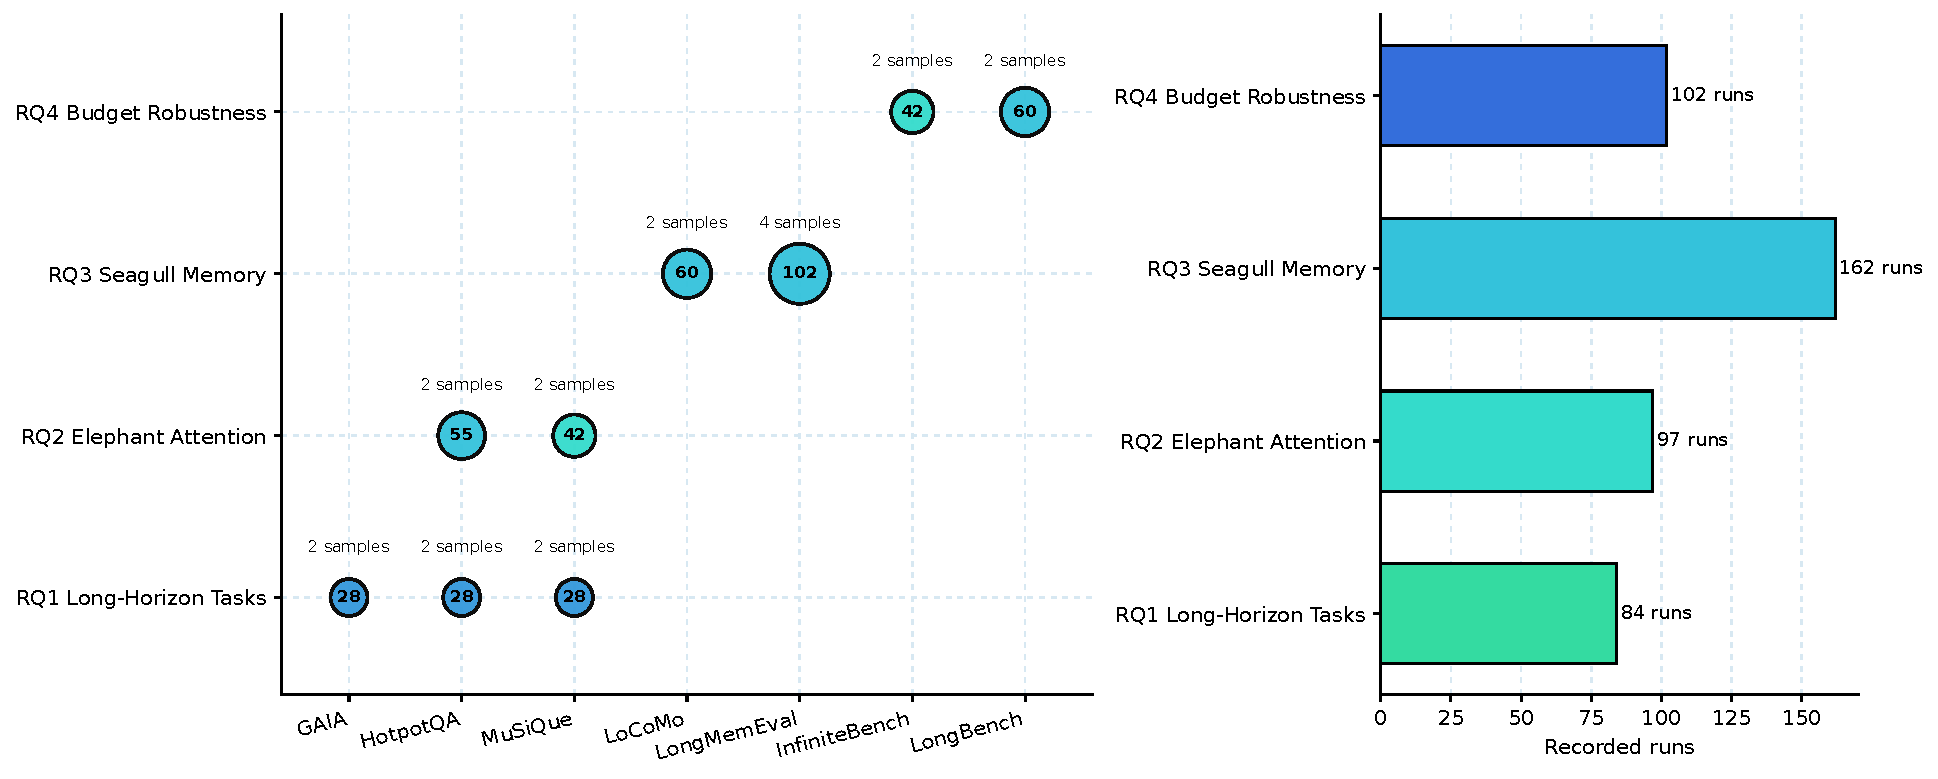
\includegraphics[width=0.98\linewidth]{experiments/report_assets/formal_coverage_map.pdf}
\caption{公开 benchmark 的覆盖密度与证据强度概览。左侧气泡大小表示 runs，颜色深浅表示真实模型数量；右侧汇总条形图展示各研究问题的总运行密度。}
\label{fig:coverage-map}
\end{figure}

为避免实验部分只给出零散数字而缺少证据结构，本节在数值表之外增加三类视觉材料。首先，图~\ref{fig:coverage-map} 给出公开 benchmark 的覆盖密度与证据强度概览，用来说明为什么不同研究问题能承载的结论强度并不相同。可以看到，RQ1 的 benchmark、模型与运行密度都明显高于其余问题，因此它更接近主证据形态；RQ2--RQ4 虽然已经通过补跑获得更好的 seed 覆盖，但密度仍不均匀，RQ5 则本质上仍是诊断性补充证据。这种“先看证据密度，再看实验优劣”的顺序，有助于让后续图表解读不脱离真实覆盖边界。

\begin{figure}[t]
\centering
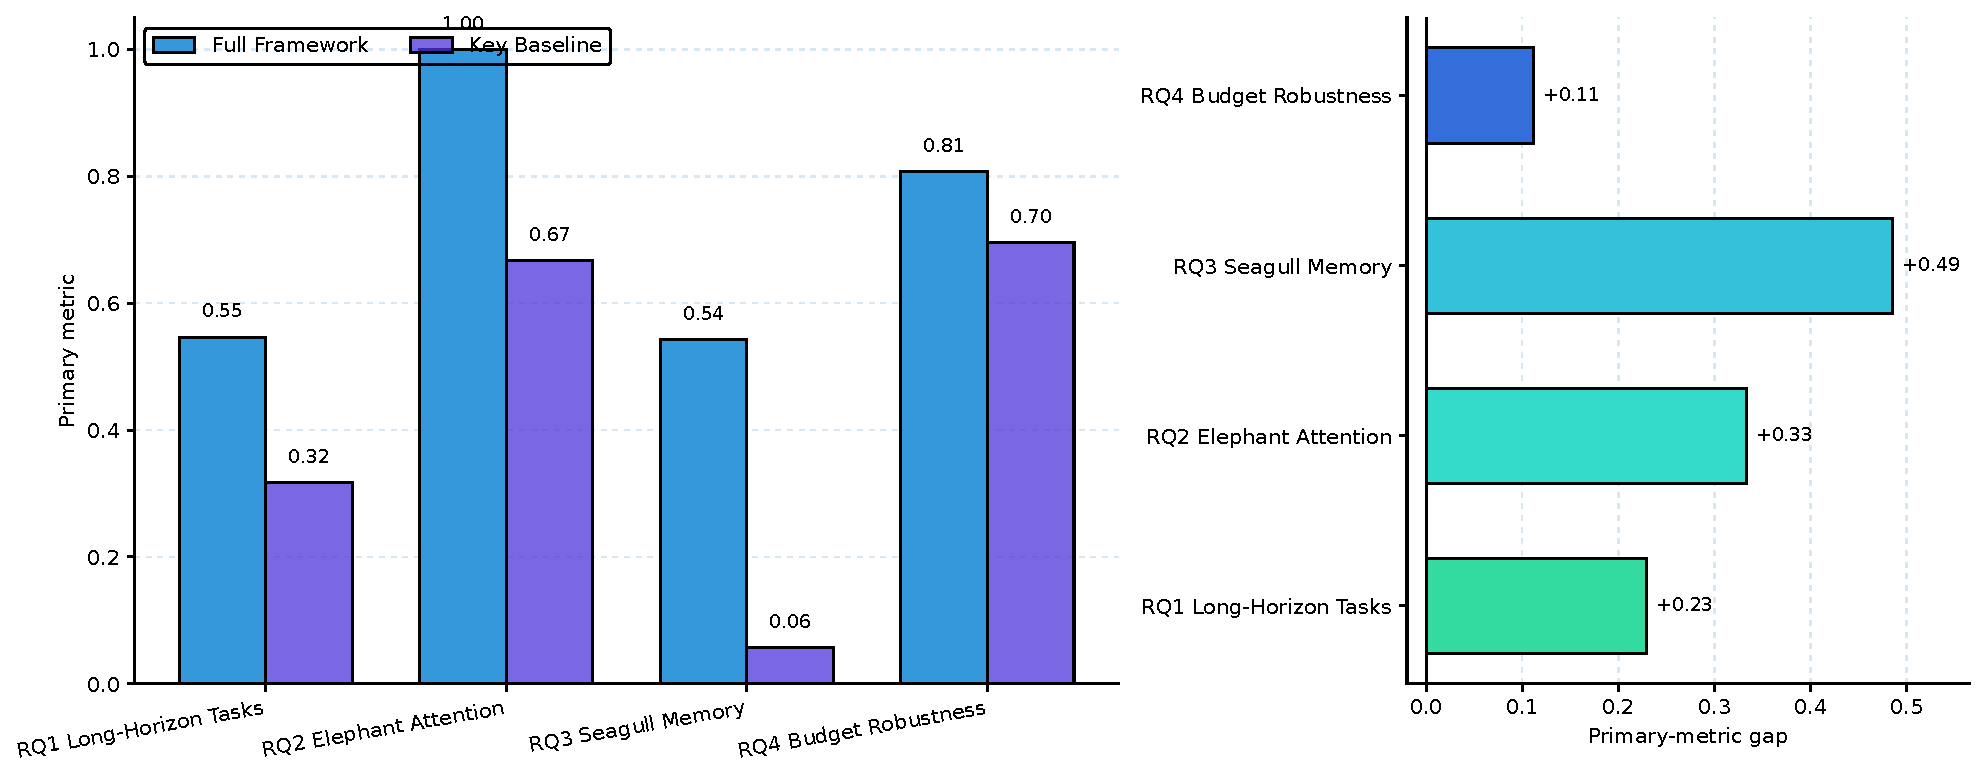
\includegraphics[width=0.98\linewidth]{experiments/report_assets/formal_main_results.pdf}
\caption{公开 benchmark 主结果。左侧展示当前仓库对齐切片上的 \texttt{full\_framework} 与关键基线的绝对主指标均值，右侧展示对应的配对差值。}
\label{fig:main-results}
\end{figure}

图~\ref{fig:main-results} 是主文最重要的公开 benchmark 结果图。左侧的绝对结果说明，RQ1 与 RQ4 中完整框架相对关键基线的优势最清晰；右侧的配对差值进一步压缩了阅读成本，使“增益来自哪里”不再只依赖表格查找。从当前结果看，RQ1 和 RQ4 的正向信号最稳定，RQ2 在本轮补跑后仍保留正向配对 gap，但优势明显弱于 RQ1 与 RQ4；RQ3 则在当前真实数据上依然没有形成正向优势。也正因为图~\ref{fig:coverage-map} 已经显示不同研究问题的证据密度并不对称，所以这里更合适的写法是：统一框架在长时程任务和预算鲁棒性上表现更好，而 RQ2 更接近“存在弱正向趋势但证据尚不闭合”，并不意味着所有模块贡献都已经被同等强度地验证。

\begin{figure}[t]
\centering
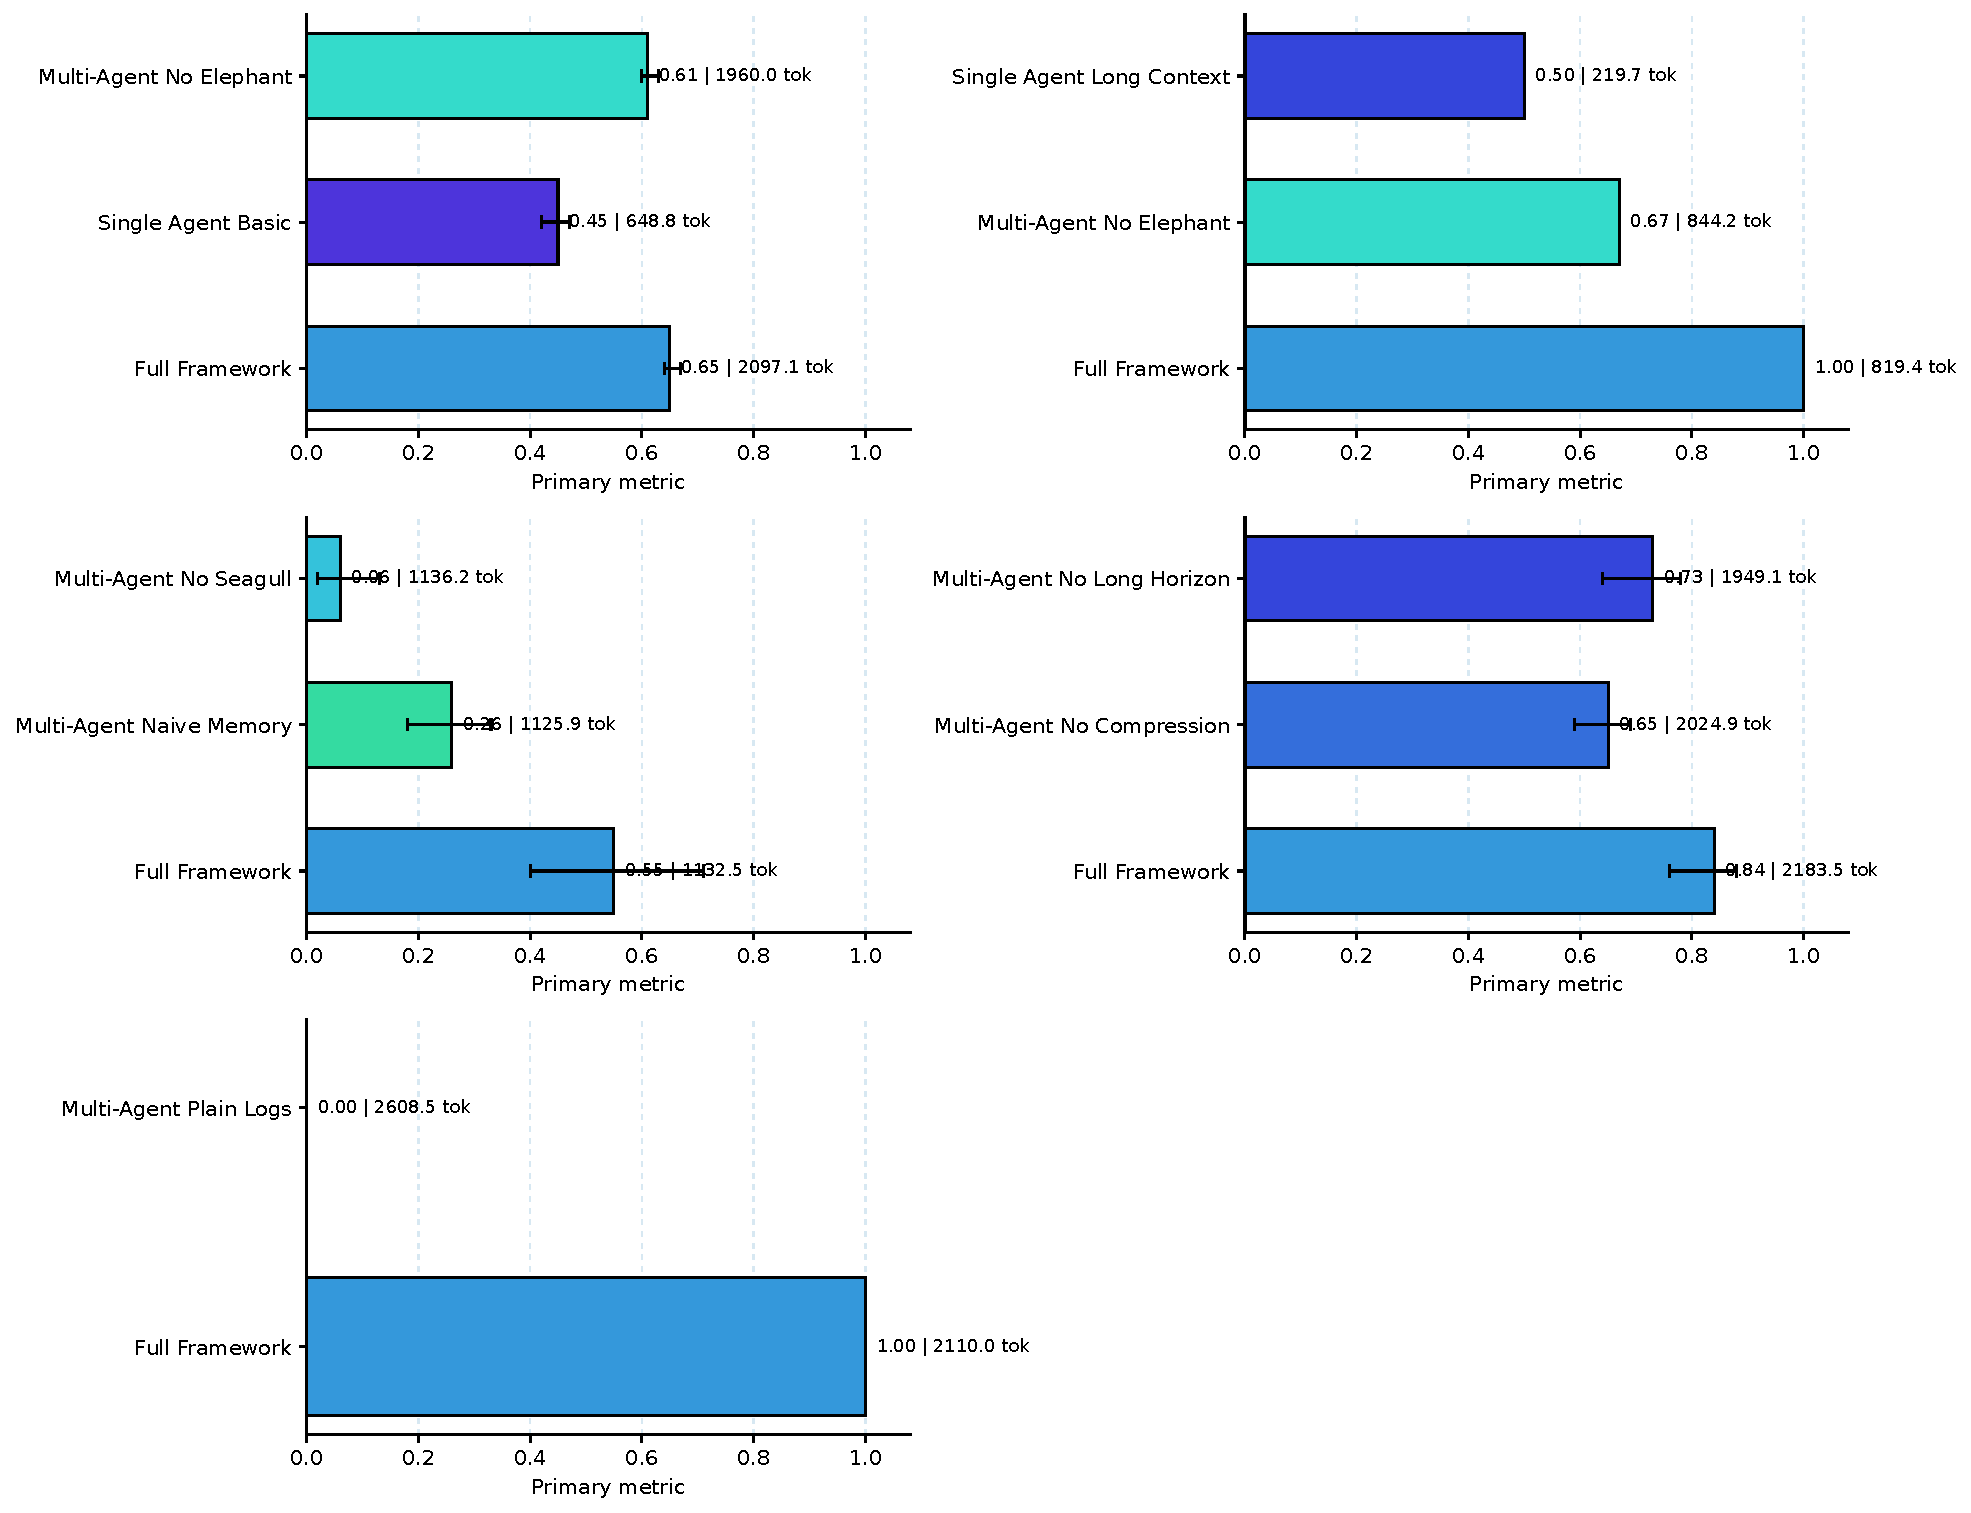
\includegraphics[width=0.98\linewidth]{experiments/report_assets/formal_reference_profile.pdf}
\caption{参考模型的实验剖面图。每个子图展示 \texttt{gpt-4o} 在对应研究问题上的绝对主指标、置信区间与 token 开销，用于观察“高分是否伴随更高成本”以及“哪些任务已接近饱和”。}
\label{fig:reference-profile}
\end{figure}

图~\ref{fig:reference-profile} 补足了只看总体均值时容易遗漏的绝对形态。它显示，在参考模型上，RQ2 与 RQ3 的多个变体都已经接近高分区间，这意味着它们的比较更容易受到 ceiling effect 的影响；同时，部分看似接近的结果其实伴随着不同的 token 使用量，说明“谁更强”之外还应关心“谁以何种成本达到相近表现”。这种剖面视角使实验叙事从单一优劣判断扩展到“绝对水平、置信区间、开销结构”三者并读，也更符合长时程系统论文应有的呈现方式。

\begin{figure}[t]
\centering
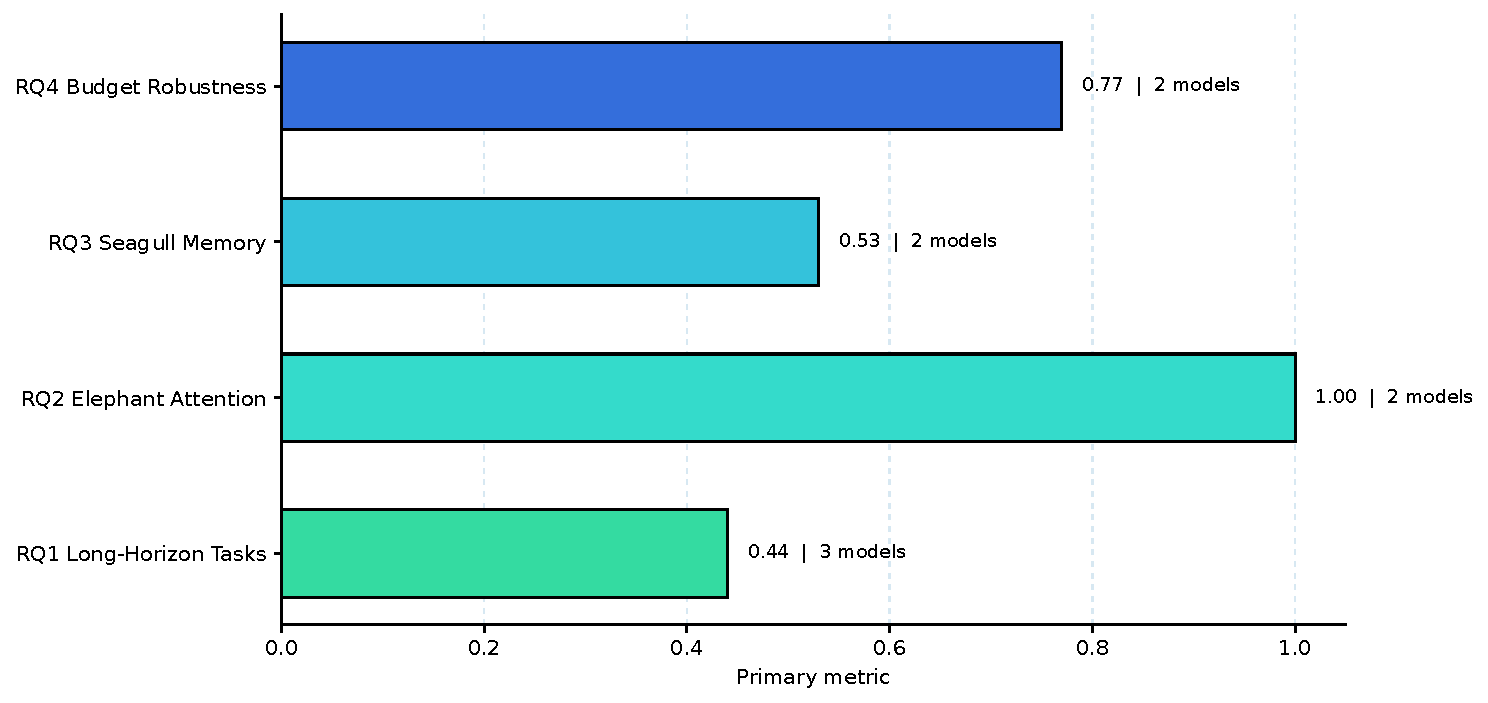
\includegraphics[width=0.94\linewidth]{experiments/report_assets/formal_cheap_model_results.pdf}
\caption{低成本真实模型聚合结果。该图用于检验收益方向是否跨模型保持，而不是证明低成本模型的绝对上限。}
\label{fig:cheap-results}
\end{figure}

图~\ref{fig:cheap-results} 展示的是低成本真实模型聚合结果。它说明，在当前已收集的公开 benchmark 仓库切片上，RQ1 与 RQ4 的收益方向并不只出现在参考模型 \texttt{gpt-4o} 上，而是在低成本模型集合中也保持为正。RQ2 的低成本模型聚合结果依旧偏向 \texttt{full\_framework}，说明大象注意力在高干扰上下文中的作用并非完全不可见，但这种趋势目前仍建立在有限模型覆盖之上。与此同时，这张图也保留了负面与不充分发现：RQ2 虽然出现了正向均值差距，但 sign test 的结果仍未达到足够稳健的统计支持，跨模型一致性也只在少数模型上成立，而且低成本单智能体长上下文基线目前仍只有一个真实模型；RQ3 则依旧没有出现预期中的正向间隔。因此，图~\ref{fig:cheap-results} 只能支持“部分模块收益具有一定跨模型迁移性”，不能支持“所有模块在不同模型上都一致成立”。

\begin{figure}[t]
\centering
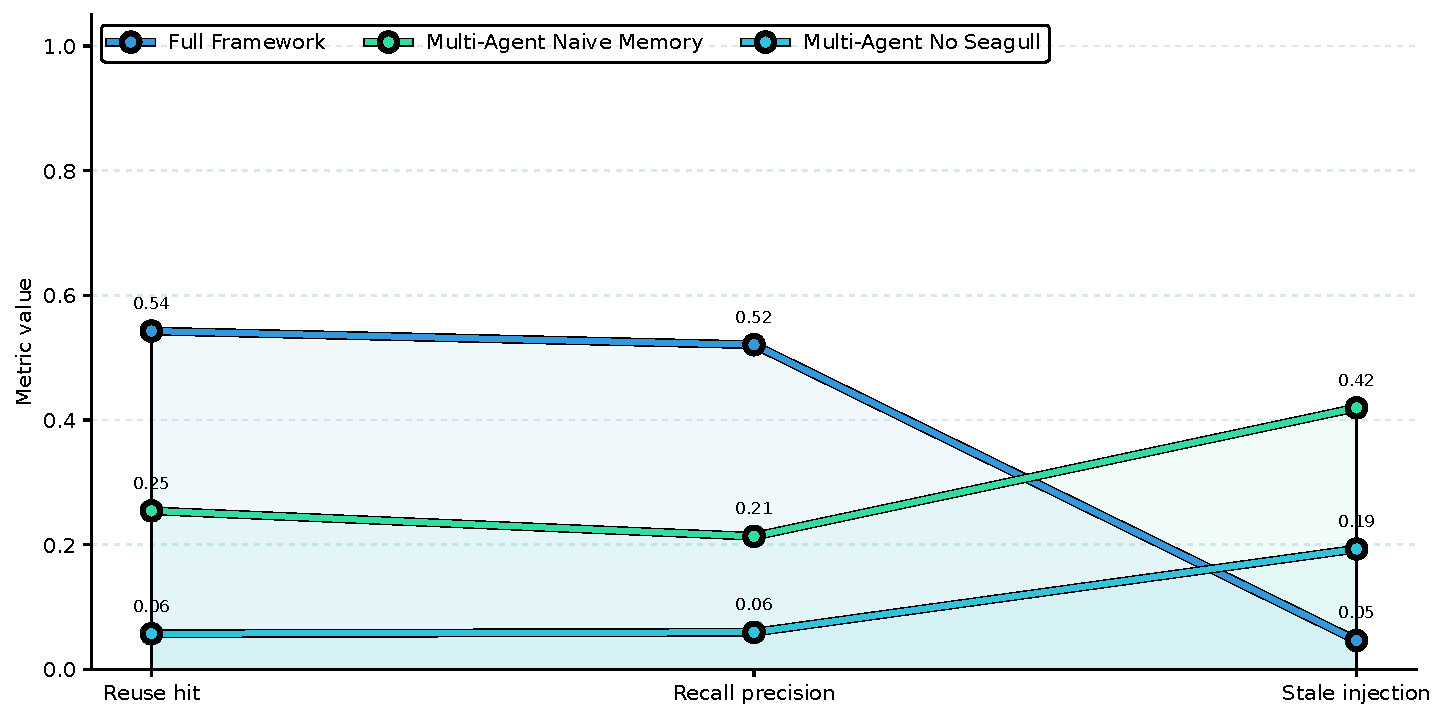
\includegraphics[width=0.90\linewidth]{experiments/report_assets/formal_rq3_memory.pdf}
\caption{RQ3 记忆诊断图。关键观察是 recall、reuse 与 stale memory 是否同时改善，而不是单一指标的局部升高。}
\label{fig:memory-diagnostics}
\end{figure}

图~\ref{fig:memory-diagnostics} 对应 RQ3。该图不再只把三个指标并排堆成静态柱状，而是强调 recall、reuse 与 stale memory 必须被联立理解。当前公开 benchmark 切片上的真实结果仍然不能支持“星鸦长时记忆图谱机制已经显著更强”这一强断言：\texttt{full\_framework} 在 recall 与 reuse 上并未明显拉开与退化变体的距离，stale memory 指标也没有形成足够清晰的优势。然而，表~\ref{tab:ltmg-baseline-aggregate} 与表~\ref{tab:ltmg-stability-aggregate} 给出的模块级强基线 benchmark 提供了更细粒度的证据。与 \texttt{vector\_memory} 和 \texttt{naive\_graph\_memory} 相比，完整图谱机制在单次聚合结果中把 \texttt{relation\_hit\_rate} 提升到 0.0324，并把 \texttt{stale\_node\_injection\_rate} 压到 0；在五个 seed 的稳定性汇总中，\texttt{conflict\_resolution\_success} 的均值为 0.9833，且 95\% 置信区间达到 [0.9500, 1.0000]。但它在 \texttt{capsule\_recall@k}、\texttt{subgraph\_relevance} 和 \texttt{returned\_memory\_usefulness} 上仍落后于 \texttt{flat\_summary\_memory}。因此，更准确的写法是：当前图谱层已经开始显示出结构化关系返回与错误记忆抑制方面的机制优势，并在多 seed 汇总下保持了相同趋势，但首屏召回排序与节点选择仍不足以支持“全面优于强基线”的结论。

\begin{figure}[t]
\centering
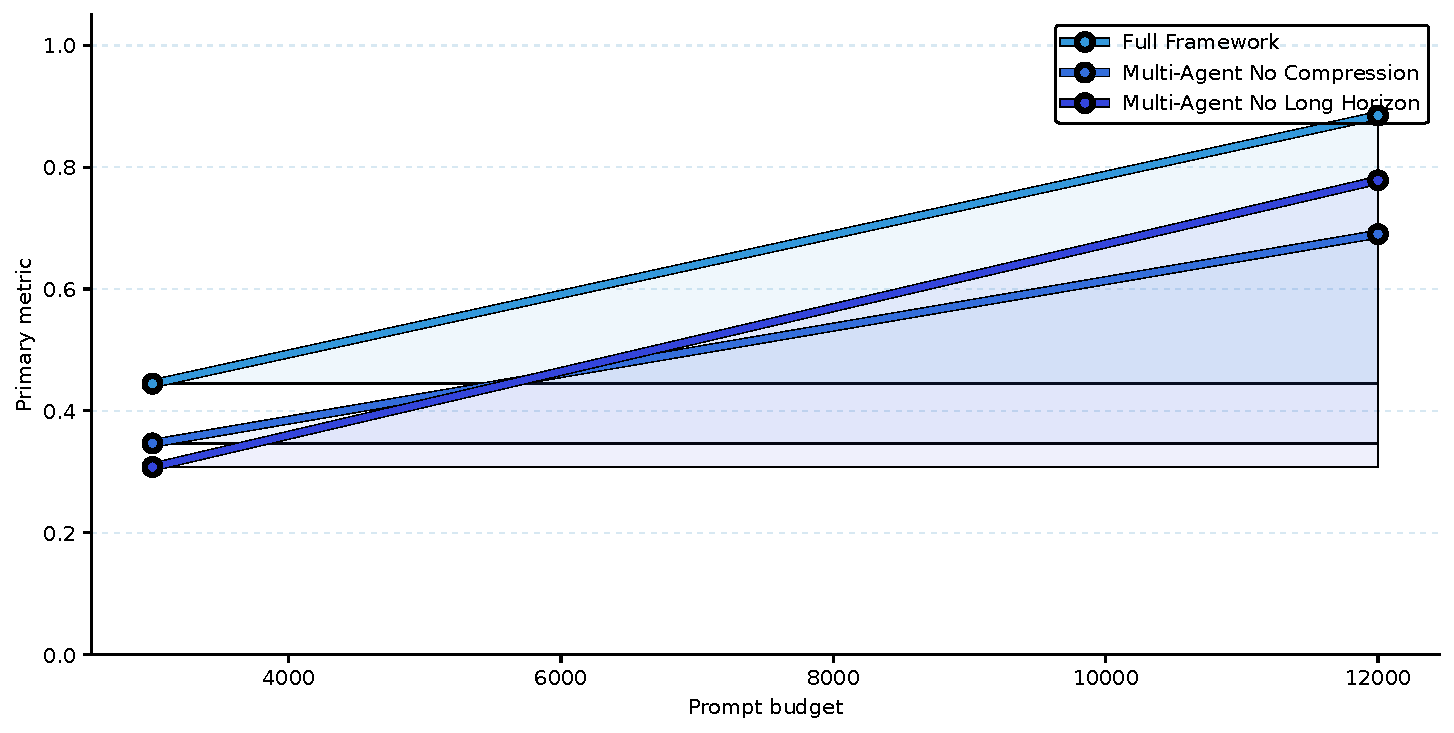
\includegraphics[width=0.94\linewidth]{experiments/report_assets/formal_rq4_robustness.pdf}
\caption{RQ4 预算鲁棒性曲线。主文关注的是预算收缩时的退化趋势，而不是某个预算点的单次高低。}
\label{fig:budget-robustness}
\end{figure}

图~\ref{fig:budget-robustness} 对应 RQ4。图中最重要的信息不是某一个预算点的绝对高低，而是预算继续收缩时各方法的退化速度。从当前真实结果看，\texttt{full\_framework} 相对于 \texttt{multi\_agent\_no\_long\_horizon} 和 \texttt{multi\_agent\_no\_compression} 维持了更高的主指标，配对差值也稳定为正。这支持了这样一种更谨慎的解释：在当前 LongBench 与 InfiniteBench 的仓库切片上，长时程注意力与上下文压缩的组合能够减缓预算压力下的性能坍塌。

不过，这一结论仍然需要受限表述。当前公开结果主要来自 LongBench 的官方子集切片，样本量和 seed 数都偏小，因此它更接近“当前切片上显示出较平缓退化曲线”，而不是“已在完整长上下文 benchmark 上稳定证明”的结论。文中所有关于预算鲁棒性的说法都应理解为这一边界下的判断。

\begin{figure}[t]
\centering
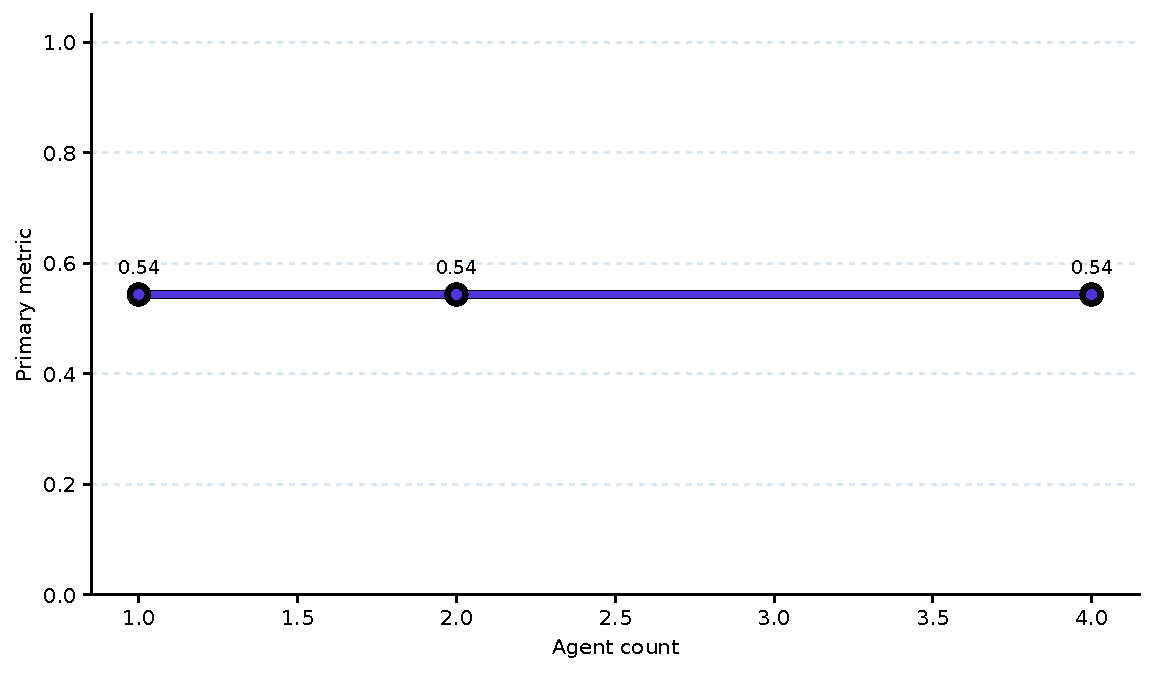
\includegraphics[width=0.86\linewidth]{experiments/report_assets/formal_scaling_curve.pdf}
\caption{补充性的扩展性结果。更多 agent 并不自动带来更强性能，因此该图只作为机制补充证据。}
\label{fig:scaling}
\end{figure}

图~\ref{fig:scaling} 是扩展性补充图，而不是主结论图。它提示我们，更多 agent 并不会自动转化为更高分数；一旦协作规模扩大，协调质量、上下文传递与记忆治理就会成为新的瓶颈。因此，这张图的价值在于说明“协作规模需要治理”，而不在于证明“增加 agent 数量本身就是优势来源”。

\subsection{跨模型结果}

跨模型分析的意义在于回答一个更窄但非常关键的问题：当前观察到的收益是否依赖某一个特别强的模型。从现有真实数据看，可以支持的说法是“部分结论具有一定方向稳定性”，尤其体现在 RQ1 与 RQ4；RQ2 在补跑后仍保留弱正向趋势，但这种趋势既没有在参考模型上清晰拉开，也没有形成充分的跨模型一致性；RQ3 则依旧只呈现混合方向，而不能支持稳定收益。也就是说，框架表现出的并不是完全统一的泛化图景，而是若干模块已经出现了可迁移的正向信号，另一些模块则仍需更大规模补跑验证，甚至可能需要重新审视模块本身的设计假设。

\begin{figure}[t]
\centering
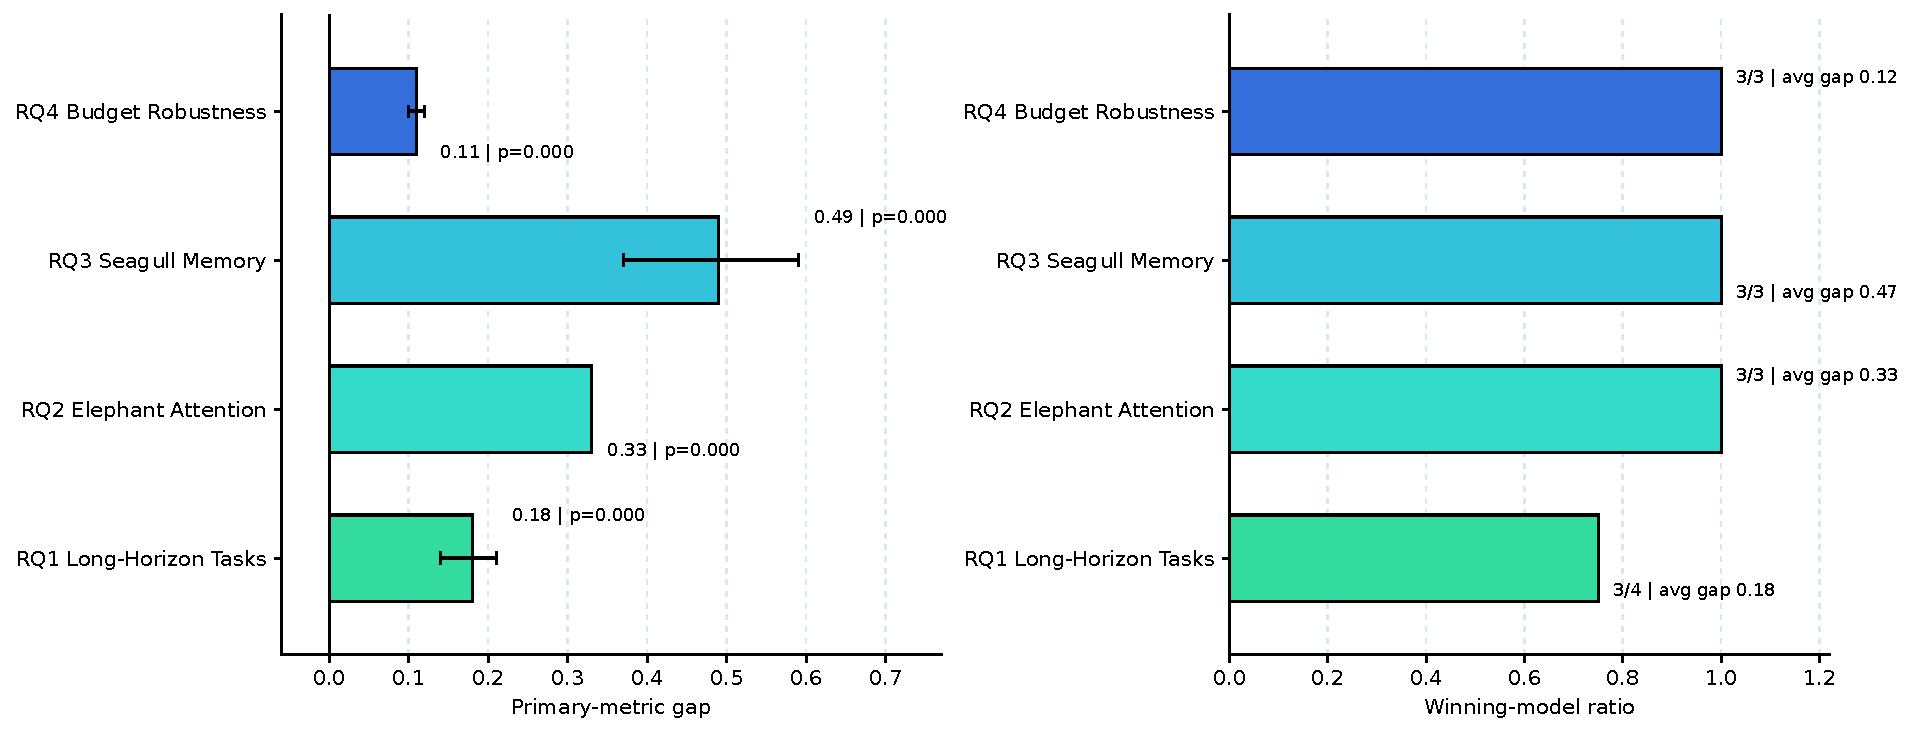
\includegraphics[width=0.98\linewidth]{experiments/report_assets/formal_gap_consistency.pdf}
\caption{配对差值与跨模型一致性联合图。左侧报告完整框架相对于关键基线的配对差值及其 bootstrap 区间，右侧报告在真实模型集合中的方向一致性。}
\label{fig:gap-consistency}
\end{figure}

图~\ref{fig:gap-consistency} 把此前分散在表格中的两个关键信号放到同一张图里：一是完整框架相对于关键基线的配对差值，二是这种差值是否在不同真实模型上保持方向一致。联合观察后，RQ1 与 RQ4 的优势比只看均值时更有说服力，因为它们既有正向配对 gap，也有较高的一致性；RQ2 虽然均值略偏正，但无论是配对区间还是方向一致性都还不够稳健；RQ3 的结果则进一步说明，当前并不能把星鸦长时记忆图谱机制写成稳定成立的模块收益；现有实验更接近对 legacy capsule-based precursor 的验证，而非对完整图谱层的闭合证据。与图~\ref{fig:main-results} 和图~\ref{fig:cheap-results} 相比，这张图更适合承担“结论边界控制”的角色。

\subsection{诊断与定性分析}

正式基准层之外，本文还保留了一条补充性诊断轨道。每次正式运行都会记录运行事件、todo 投影、记忆治理信号、上下文选择轨迹与逐样本执行元数据，因此框架的评估不再只关心一个变体是否成功，也关心其成功或失败是否可被结构化解释。这里需要再次强调的是：这类结果承担的是机制说明作用，而不是公开 benchmark 级主结论。

\begin{figure}[t]
\centering
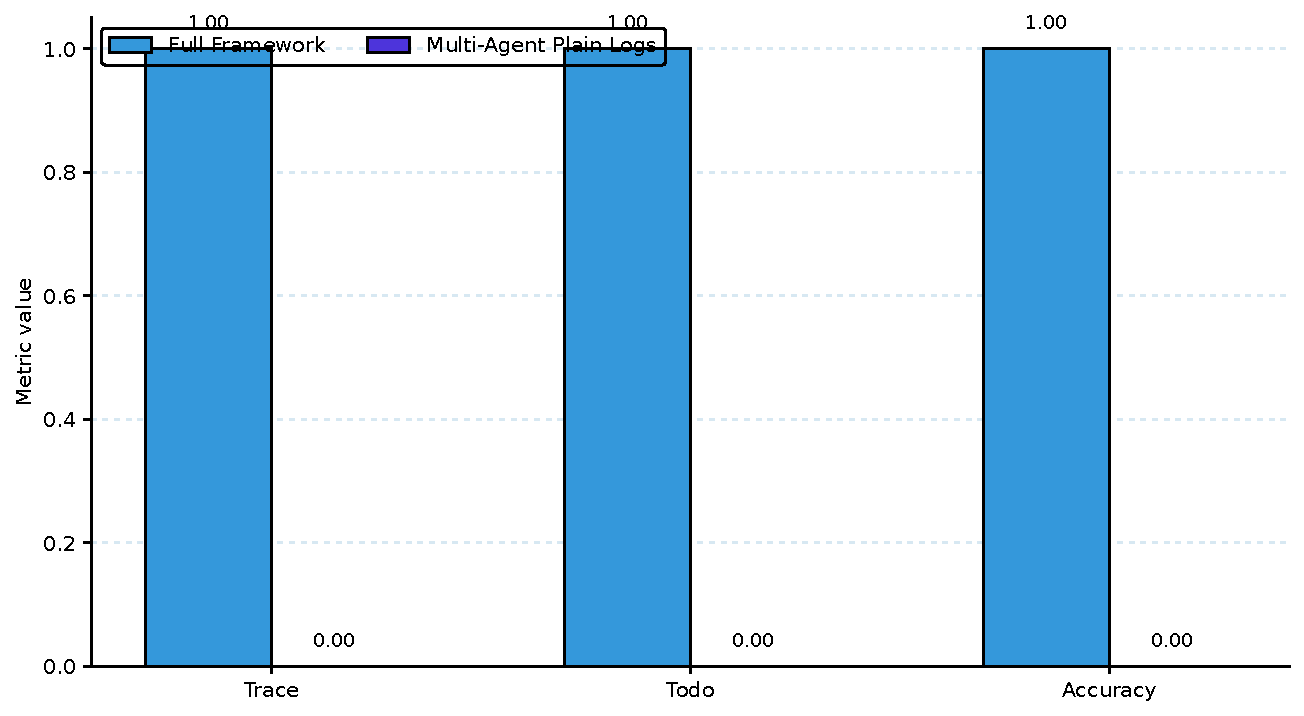
\includegraphics[width=0.90\linewidth]{experiments/report_assets/formal_failure_breakdown.pdf}
\caption{补充性的 RQ5 诊断结果。可观测性图用于解释轨迹覆盖与故障定位能力，不承担公开 benchmark 级主结论。}
\label{fig:failure-breakdown}
\end{figure}

图~\ref{fig:failure-breakdown} 展示了 RQ5 的补充诊断结果。这里最重要的不是 Failure Suite 上的总体 \texttt{quality\_score}，因为该指标在当前小样本切片上接近饱和；真正有解释力的是轨迹覆盖率、todo 一致性和诊断准确率等可观测性指标。结果说明，事件中心可观测性有助于形成更可重建的任务轨迹，从而提高故障定位能力，但这类结果目前只应被看作机制性补充证据，而不能替代公开 benchmark。

\subsection{多智能体多轮对话分析}

多智能体多轮对话是一个有解释力但证据等级较低的压力测试，因为它同时要求系统保留早期约束、维持委派连续性，并在后续轮次中吸收新需求而不丢失已有结构。这恰好对应大象注意力、星鸦长时记忆图谱机制、长时程注意力与上下文压缩需要协同工作的场景，也说明两篇章节论文在系统层确实存在互补关系。

\begin{figure}[t]
\centering
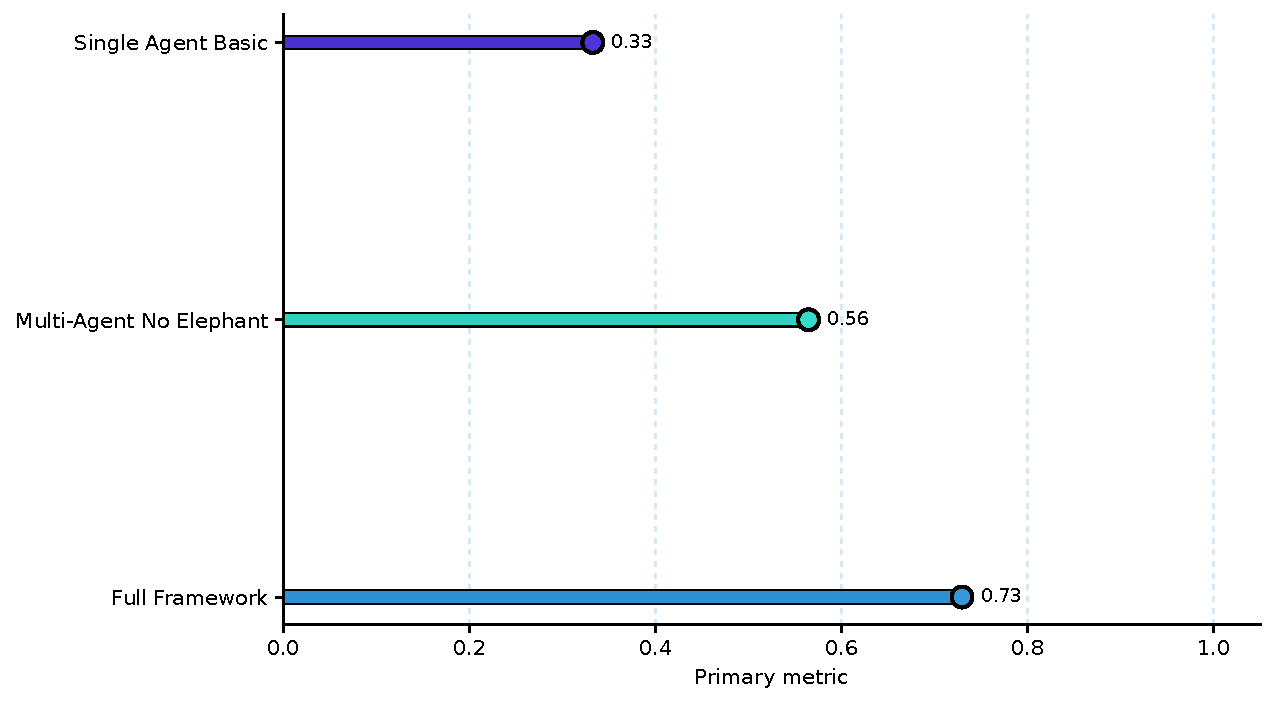
\includegraphics[width=0.94\linewidth]{experiments/report_assets/formal_multiturn_results.pdf}
\caption{补充性的多轮对话结果。该图用于说明跨轮连续性与委派保持，而非主文核心 benchmark 结论。}
\label{fig:multiturn}
\end{figure}

图~\ref{fig:multiturn} 展示了多轮对话补充结果。它表明，在 AgentOrch MultiTurn Suite 这一专门构造的连续性环境中，完整框架比去除大象注意力或退化为单智能体更容易保持跨轮约束与委派连续性。这一现象与 RQ1 中观察到的长时程协作收益在方向上相容，但由于该套件不是公开 benchmark，且当前覆盖仍小，因此本文只把它作为辅助解释材料。

\section{结果讨论}

综合以上结果，当前真实数据能够支持三类较为稳健的判断。第一，统一框架在公开 benchmark 的长时程任务上优于单智能体强退化基线，尤其体现在 RQ1。第二，在当前仓库对齐切片上，长时程注意力与上下文压缩组合显示出更清晰的正向预算鲁棒性信号。第三，大象注意力在高干扰上下文中的收益只呈现弱正向趋势，现阶段更适合被描述为“证据未闭合但方向略偏正”而非稳定结论。事件中心可观测性与多轮连续性结果则继续作为机制补充，帮助解释为什么该框架更适合长时程协作任务。

与此同时，本文也必须保留几类明确的负面或不充分发现。RQ2 虽然出现了正向 gap，但统计显著性和跨模型一致性仍不足，而且参考模型结果并未与低成本聚合结果一起形成清晰分离，因此不能把它写成稳定成立的模块收益。RQ3 的证据更需要区分两个层次：在公开 benchmark 切片上，完整框架尚未对历史退化变体形成稳定正向优势，因此不能直接把星鸦机制写成成熟收益；在新增的模块级强基线 benchmark 中，当前图谱实现虽然已经在关系命中、陈旧抑制和冲突消解上优于 \texttt{vector\_memory} 与 \texttt{naive\_graph\_memory}，但仍未在首屏 recall、relevance 和 usefulness 上超过 \texttt{flat\_summary\_memory}。这说明当前机制离“全面优于强基线”的投稿口径还有距离，更准确的表述应是：完整图谱机制已经显示出结构化子图返回与安全控制方面的机制优势，但召回排序与首屏选择仍需继续优化。部分图表中的高成功率对应的实际样本量仍然偏小，因此不能被表述为大规模稳定现象。换句话说，当前稿件更接近一篇“公开 benchmark 主导、真实数据驱动、但结论边界严格受控”的方法论文，而不是已经完成全面优越性证明的成熟 benchmark 论文。

\section{局限性}

当前稿件有意对尚未完成的部分保持诚实。最重要的限制首先来自证据覆盖边界：主文中的若干 benchmark 仍是仓库内置的对齐切片，而非完整公开 benchmark；真实模型调用成本与运行时间也继续限制 benchmark 覆盖范围，因此即使本轮已把 RQ2--RQ4 的参考模型核心对照补到五个 seed，模型与 benchmark 的覆盖仍然不均匀。其次，主要任务质量指标依赖 judge-based 评分，这可能引入评价偏差，人工评审与双盲复核仍需补充。再次，自定义诊断套件只能作为补充证据，不能替代公开 benchmark 去支撑主结论；当前跨模型分析也仍局限于少量真实模型，尚不足以支撑更强的跨提供商泛化陈述。最后，成本-性能权衡、失败类型附录以及更大规模多 seed 复现实验都还没有扩展到投稿级完整度。

这些局限之所以重要，是因为方法论文的说服力并不来自概念新颖本身，而来自“概念、实验协议、统计汇总与结论边界”四者之间是否严格一致。因此，当前版本更适合被理解为一个已经具备真实 benchmark 主证据的高强度稿件雏形，而不是已经完成全部验证的最终优越性证明。

此外，该方法本身也存在风险。若系数校准不当，大象注意力可能会过度偏向历史上已验证的信息，从而抑制真正有价值的新证据。若提升、构边与返回阈值设置过于宽松，克拉克星鸦长时记忆图谱机制仍可能积累陈旧节点、错误关系或冲突子图。长时程注意力依赖摘要与状态快照算子的质量，而这些算子本身也可能引入失真。若冗余抑制调节不佳，上下文压缩可能会丢弃那些低频但决定性的证据。最后，事件中心可观测性虽然提升了可解释性，但也引入了额外的存储与实现开销，未来需要显式测量。

\section{结论}

本文将长时程多智能体大语言模型系统重新表述为一个统一的治理问题，而不是若干工程模块的临时拼装。所提出的大象-星鸦框架把大象注意力、克拉克星鸦长时记忆图谱机制、长时程注意力、上下文压缩、MGCM 与事件中心可观测性组织为一组可联合分析的机制，用于共同治理上下文、记忆、协作与进度重建。其中，大象注意力与星鸦图谱机制分别对应两篇可独立展开的章节论文，而第五章系统实验则负责验证两者的耦合增益。

基于当前真实结果，本文能够得出的结论是审慎而明确的：统一框架在公开 benchmark 的长时程任务上相对单智能体强退化基线表现更好，并在预算鲁棒性上显示出较清晰的正向信号；与此同时，大象注意力在高干扰上下文中的收益目前只表现为弱正向趋势，尚未达到稳定结论的强度，星鸦长时记忆图谱机制的独立贡献则在当前 bundled slice 上未见稳定优势，仍需更大规模、更多 seed 与更完整 benchmark 覆盖来进一步验证。更严格地说，当前仓库只提供了对 legacy capsule-based precursor 的实现级与弱效能级证据，而完整图谱机制仍属于待系统验证的正式模块。补充性的诊断与多轮结果为机制解释提供了支持，但不应被误读为主 benchmark 级证据。

因此，本文的主要价值在于给出了一套已经能被真实数据部分支持、且能继续扩展的统一实验与方法框架。下一步工作应集中于补齐公开 benchmark 覆盖、完成五 seed 正式协议、增加人工评审与更强统计检验，并在不改变核心方法表述的前提下，把当前稿件推进到更接近正式投稿的证据强度。

\begin{thebibliography}{00}

\bibitem[Chan et~al.(2024)]{chan2024chateval}
Chan, C.-M., Chen, W., Su, Y., Yu, J., Xue, W., Zhang, S., et al., 2024. ChatEval: Towards better LLM-based evaluators through multi-agent debate. In: International Conference on Learning Representations. \url{https://openreview.net/forum?id=FQepisCUWu}.

\bibitem[Dong et~al.(2026)]{dong2026pear}
Dong, Z., Li, Y., Zhang, J., Li, Y., Ye, X., Sui, P., et al., 2026. PEAR: Plan, execute, assess, and refine: A robust planner-executor-agent benchmark. In: Findings of the Association for Computational Linguistics: EACL 2026, 3458--3477. \url{https://aclanthology.org/2026.findings-eacl.237/}.

\bibitem[Du et~al.(2025)]{du2025crossteam}
Du, Z., Qian, C., Liu, W., Xie, Z., Wang, Y., Dang, Y., et al., 2025. Multi-Agent Collaboration via Cross-Team Orchestration. In: Findings of the Association for Computational Linguistics: ACL 2025, 10566--10584. \url{https://aclanthology.org/2025.findings-acl.541/}.

\bibitem[Gan et~al.(2025)]{gan2025master}
Gan, B., Shi, W., Li, X., Kong, M., Xu, S., Wang, W., et al., 2025. MASTER: A multi-agent system with LLM specialized MCTS. In: Proceedings of the 2025 Conference of the North American Chapter of the Association for Computational Linguistics: Human Language Technologies, 9570--9594. \url{https://aclanthology.org/2025.naacl-long.476/}.

\bibitem[Guo et~al.(2024)]{guo2024llmmas}
Guo, T., Chen, X., Wang, Y., Chang, R., Pei, S., Chawla, N. V., et al., 2024. Large language model based multi-agents: A survey of progress and challenges. In: Proceedings of the Thirty-Third International Joint Conference on Artificial Intelligence, 8048--8057. \url{https://doi.org/10.24963/ijcai.2024/890}.

\bibitem[Hong et~al.(2024)]{hong2024metagpt}
Hong, S., Zhuge, M., Chen, J., Zheng, X., Cheng, Y., Zhang, C., et al., 2024. MetaGPT: Meta-programming for a multi-agent collaborative framework. In: International Conference on Learning Representations. \url{https://openreview.net/forum?id=VtmBAGCN7o}.

\bibitem[Li et~al.(2023)]{li2023camel}
Li, G., Hammoud, H. A. A. K., Itani, H., Khizbullin, D., Ghanem, B., 2023. CAMEL: Communicative agents for ``mind'' exploration of large scale language model society. In: Advances in Neural Information Processing Systems 36. \url{https://proceedings.neurips.cc/paper_files/paper/2023/hash/a3621ee907def47c1b952ade25c67698-Abstract-Conference.html}.

\bibitem[Li et~al.(2024a)]{li2024sbarope}
Li, R., Xu, J., Cao, Z., Zheng, H.-T., Kim, H.-G., 2024. Extending context window in large language models with segmented base adjustment for rotary position embeddings. Applied Sciences 14, 3076. \url{https://doi.org/10.3390/app14073076}.

\bibitem[Li et~al.(2024b)]{li2024masworkflow}
Li, X., Wang, S., Zeng, S., Wu, Y., Yang, Y., 2024. A survey on LLM-based multi-agent systems: Workflow, infrastructure, and challenges. Vicinagearth 1, 100007. \url{https://doi.org/10.1007/s44336-024-00009-2}.

\bibitem[Liu et~al.(2024)]{liu2024agentbench}
Liu, X., Yu, H., Zhang, H., Xu, Y., Lei, X., Lai, H., et al., 2024. AgentBench: Evaluating LLMs as agents. In: International Conference on Learning Representations. \url{https://openreview.net/forum?id=zAdUB0aCTQ}.

\bibitem[Lewis et~al.(2020)]{lewis2020rag}
Lewis, P., Perez, E., Piktus, A., Petroni, F., Karpukhin, V., Goyal, N., Kuttler, H., Lewis, M., Yih, W.-t., Rocktaschel, T., Riedel, S., Kiela, D., 2020. Retrieval-augmented generation for knowledge-intensive NLP tasks. Advances in Neural Information Processing Systems 33, 9459--9474.

\bibitem[Park et~al.(2023)]{park2023generative}
Park, J. S., O'Brien, J. C., Cai, C. J., Morris, M. R., Liang, P., Bernstein, M. S., 2023. Generative agents: Interactive simulacra of human behavior. In: Proceedings of the 36th Annual ACM Symposium on User Interface Software and Technology, 1--22. \url{https://doi.org/10.1145/3586183.3606763}.

\bibitem[Qian et~al.(2024)]{qian2024chatdev}
Qian, C., Liu, W., Liu, H., Chen, N., Dang, Y., Li, J., et al., 2024. ChatDev: Communicative agents for software development. In: Proceedings of the 62nd Annual Meeting of the Association for Computational Linguistics (Volume 1: Long Papers), 14927--14956. \url{https://aclanthology.org/2024.acl-long.810/}.

\bibitem[Qian et~al.(2025)]{qian2025macnet}
Qian, C., Liu, W., Lu, Y., Wei, Y., Du, Z., Yang, C., et al., 2025. Scaling large language model-based multi-agent collaboration. In: International Conference on Learning Representations. \url{https://openreview.net/forum?id=K3n5jPkrU6}.

\bibitem[Shinn et~al.(2023)]{shinn2023reflexion}
Shinn, N., Cassano, F., Gopinath, A., Narasimhan, K., Yao, S., 2023. Reflexion: Language agents with verbal reinforcement learning. In: Advances in Neural Information Processing Systems 36. \url{https://proceedings.neurips.cc/paper_files/paper/2023/hash/1b44b878bb782e6954cd888628510e90-Abstract-Conference.html}.

\bibitem[Wang et~al.(2024a)]{wang2024survey}
Wang, L., Ma, C., Feng, X., Zhang, Z., Yang, H., Zhang, J., Chen, Z., Tang, J., Chen, X., Lin, Y., Zhao, W. X., Wei, Z., Wen, J., 2024. A survey on large language model based autonomous agents. Frontiers of Computer Science 18, 186345. \url{https://doi.org/10.1007/s11704-024-40231-1}.

\bibitem[Wang et~al.(2024b)]{wang2024sotopiapi}
Wang, R., Zhou, X., Li, Y., Brahman, F., Tan, C., Liu, Z., et al., 2024. SOTOPIA-$\pi$: Interactive learning of socially intelligent language agents. In: Proceedings of the 62nd Annual Meeting of the Association for Computational Linguistics (Volume 1: Long Papers), 12957--12983. \url{https://aclanthology.org/2024.acl-long.698/}.

\bibitem[Wang et~al.(2025)]{wang2025megaagent}
Wang, J., Wang, Z., Sun, L., He, K., Liu, M., Chen, A., et al., 2025. MegaAgent: Scaling large language model-based multi-agent systems without predefined workflows. In: Findings of the Association for Computational Linguistics: ACL 2025, 5031--5065. \url{https://aclanthology.org/2025.findings-acl.259/}.

\bibitem[Wooldridge(2009)]{wooldridge2009}
Wooldridge, M., 2009. An Introduction to MultiAgent Systems. Wiley, Chichester.

\bibitem[Wu et~al.(2023)]{wu2023autogen}
Wu, Q., Bansal, G., Zhang, J., Wu, Y., Li, B., Zhu, E., et al., 2023. AutoGen: Enabling next-gen LLM applications via multi-agent conversation. arXiv preprint arXiv:2308.08155. \url{https://doi.org/10.48550/arXiv.2308.08155}.

\bibitem[Yao et~al.(2023)]{yao2023react}
Yao, S., Zhao, J., Yu, D., Du, N., Shafran, I., Narasimhan, K., Cao, Y., 2023. ReAct: Synergizing reasoning and acting in language models. In: International Conference on Learning Representations. \url{https://openreview.net/forum?id=WE_vluYUL-X}.

\bibitem[Zhou et~al.(2024)]{zhou2024sotopia}
Zhou, X., Zhu, H., Mathur, L., Zhang, R., Yu, H., Qi, Z., et al., 2024. SOTOPIA: Interactive evaluation for social intelligence in language agents. In: International Conference on Learning Representations. \url{https://openreview.net/forum?id=mM7VurbA4r}.

\end{thebibliography}

\end{CJK*}
\end{document}
